%%Définir le format du document: papier, taille de police, type de document, etc.

\documentclass[11pt, french]{article}

%%%%%%%%%% Packages externes utilisés %%%%%%%%%%%%%%%%%%%
\usepackage[french]{babel}
\selectlanguage{french}
\usepackage[T1]{fontenc}
\usepackage[utf8]{inputenc}

\usepackage{verbatim}
\usepackage{graphicx}
\usepackage{epstopdf}
\usepackage{macro}
\usepackage{algorithm}
\usepackage{algorithmic}
%\usepackage{algorithm2e}


%La mise en page du rapport, NE PAS MODIFIER.
\usepackage{geometry}
 \geometry{
 a4paper,
 left=20mm,
 right=20mm,
 top=20mm,
 bottom=20mm,
 }

%%%%%%%%% Le corps du document entre begin et end %%%%%%%%%%%%%%%%%%%
\begin{document}

%Page de garde
%%%%%%%%%%%%%%% Page de garde %%%%%%%%%%%%%%%%%%%

\begin{titlepage}{
    \begin{center}
        \vspace* {25mm}
        {\Large \textbf {Université de Cergy-Pontoise}} \\
        \vspace* {10mm}
        {\Large \textbf {RAPPORT}} \\
        \vspace* {10mm}
        pour le projet Génie Logiciel \\
        \textbf {Licence d'Informatique deuxième année} \\
        \vspace* {10mm}

	sur le sujet \\
        \vspace* {10mm}
	{\Huge \textsf{Football}} \\
        \vspace* {10mm}
 	rédigé par \\
        \vspace* {10mm}
        {\Large \textbf {RIEDEL Romain, LEGUAY Guillaume et CHEYNET Boyan}} \\
				\vspace* {10mm}
        \date MMars 2023
        \vspace* {10mm}
	\end{center}
}
\end{titlepage}


%Génération automatique de la table des matières, de la liste des figures et de la liste des tableaux
\tableofcontents
\listoffigures
\listoftables

%Une section "remerciements" pourrait être intéressante. C'est une section sans numérof (avec un * )

\newpage
\section* {Remerciements}
\paragraph{}
Cher Professeur,
\paragraph{}
Nous tenons à vous exprimer notre gratitude pour tout le temps et les efforts que vous avez consacrés à notre projet de génie logiciel en L2 Informatique. Votre encadrement et vos conseils précieux ont grandement contribué à la réussite de ce projet.
\paragraph{}
Votre expertise et votre passion pour le génie logiciel ont été une source d'inspiration pour nous tous. Vous avez su nous guider avec patience et nous avez permis de développer nos compétences en matière de programmation et de gestion de projet.
\paragraph{}
Nous avons tous beaucoup appris grâce à votre enseignement, vos commentaires et votre soutien continu. Votre implication et votre dévouement pour nos projets ont été inestimables et nous sommes très reconnaissants pour cela.
\paragraph{}
Je tiens également à vous remercier pour votre disponibilité et votre ouverture d'esprit tout au long du semestre. Votre encouragement et votre confiance en nous ont été très motivants et ont contribué à notre progression dans le domaine du génie logiciel.
\paragraph{}
Encore une fois, merci infiniment pour tout ce que vous avez fait pour nous. Votre influence positive continuera à se faire sentir dans nos carrières futures.

\newpage
\section{Introduction}
\label{sec:introduction}

Dans cette section, nous allons présenter brièvement de nos motivations pour le projet, l'expliquer de manière simple et introduire le reste du rapport. 


\subsection{Contexte du projet}
\paragraph{}
    Notre projet consiste à créer un jeu de simulation de football, ce qui implique la modélisation de différents aspects du sport tels que les règles, les mouvements des joueurs, la physique du ballon et l'environnement du terrain. Le but du jeu serait de permettre aux joueurs de vivre l'expérience d'un match de football en simulant un match  avec différentes tactiques. Le jeu pourrait inclure des fonctionnalités telles que la personnalisation des joueurs et des équipes, ainsi que de la compositions et de la tactique déployé.


\subsection{Objectif du projet}
\paragraph{}
    L'objectif de ce projet est la réalisation d'un jeu de football, plus précisément la simulation complexe et réaliste d'un match de football, dans laquelle l'utilisateur ne pourra que choisir son équipe, sa composition et ses joueurs au préalable du match. Néanmoins, l'utilisateur ne pourra en aucun cas interagir durant le match. Parmi les objectifs concrets, nous auront comme principales tâches le développement de deux équipes de 11 joueurs, entièrement automatisés. Chacune des actions des joueurs sera réfléchies et non-aléatoire, afin d'y obtenir un résultat réaliste, et une simulation fidèle à la réalité. De plus, chacun des arrêt de jeu tel que les fautes, les touches, etc. seront présent et incorporés dans notre jeu.

\subsection{Organisation du rapport}

\paragraph{}
    
\newpage
\section{Spécification du projet}
\label{sec:specification}

\paragraph{} Nous avons présenté l'objectif du projet dans la section \ref{sec:introduction}. Dans cette section, nous présentons la spécification de notre logiciel réalisé. Ceci correspond principalement au document de spécification du projet (cahier des charges).

\subsection{Notions de base et contraintes du projet}
\label{sec:spec1}

\paragraph{}
    Voici une liste détaillée des termes et notion importante à définir pour notre projet :


\paragraph{Règles Football :} Pour les règles, nous nous baserons sur celle des compétitions internationales.

\paragraph{Les Systèmes de jeu :} Au football, le système de jeu est une façon d’organiser les joueurs afin que ceux-ci aient des consignes spécifiques même si ces responsabilités et ces fonctions sont par essence momentanées, elles assurent une filiation avec un ensemble de lignes directrices et de règles en fonction de la rencontre à venir et des conceptions de l’entraîneur. L’utilisateur aura la possibilité de choisir parmi un ensemble fini de système. Cet ensemble contiendra majoritairement les systèmes populaires des compositions plus fantaisies. Durant la simulation, les joueurs suivront scrupuleusement ce système dans leurs placement naturel.

\paragraph{Choix stratégique :} Le système de choix stratégique intervient après le choix des différents joueurs, ce système permet de définir le type de jeu que l'équipe de l’utilisateur va suivre. Ce choix va dicter le comportement général des joueurs dans leur placement sans ballon, leur réaction à la perte ou à la récupération du ballon. Ce choix va se représenter par différentes barres à incrémenter ou non. Ces différentes barres correspondent à différentes stratégies : contre-attaque, pièges hors jeu, pressing et bloc bas.De plus, pendant ce choix, l’utilisateur devra choisir les joueurs qui tireront les corners, coups francs et penalty

\paragraph{Équipes :} Équipe composée de 11 joueurs sur le terrain. On distingue graphiquement ces équipes par des couleurs de maillots.

\paragraph{Joueurs :} Les joueurs seront générée aléatoirement avec noms et prénoms issus d’une liste et de statistiques (cf. prochain point) qui les distinguent. Cette génération se base sur une génération de 35 joueurs réparties en archétypes : 5 gardiens, 10 défenseurs, 10 attaquants et 10 milieux. Par la suite, l’utilisateur va composer son équipe en prenant compte des différences statistiques et son système puis choisir les remplaçants/titulaires.

\paragraph{Statistiques :} Les statistiques sont les représentations numériques du niveau du joueur dans certaines catégories. Elles entrent directement en compte dans la réussite d’une action (cf. prochain point). La génération aléatoire de celles ci s’effectuer comme tel : un joueur de l'archétype défenseur a une défense de base de 70 puis un nombre entre [-10;+20] sera appliquée donnant la statistique finale du joueur (les nombres ne sont absolument pas définitif, ils sont donnés à titre d’exemple).Les statistiques communes à tous les archétypes sont : défense, tir, passe, endurance, vitesse et zone d’action.Pour les gardiens, une statistique arrêt existe.

\paragraph{Fonction des statistiques :} La défense rentre en compte dans les actions défensives telles que les interceptions, les tacles et le marquage. Le tir correspond à la capacité du joueur à réussir un tir. Passe correspond au chance de réussite d’une passe. L’endurance est une statistique qui ajoute des malus dans la réalisations d’autres actions représentant la fatigue du joueur, c’est cette statistique qui va rentrer en compte lors du remplacement des joueurs. La vitesse retranscrit la vitesse de déplacement du joueur sur le terrain. La zone d’action correspond à une zone autour du joueur dans laquelle il peut tenter une action défensive. Pour les gardiens, la statistique d’arrêt est la chance que le gardien arrête le tir dans sa zone d’action. Le fonctionnement des statistiques se croisent dans le sens ou certaines vont infliger des malus dans la réalisation de certaines actions.

\paragraph{Terrain :} Le terrain sera représenté sur la majorité de l'écran et respectera les ratios d’un véritable terrain de football. Pour manipuler les positions des éléments, le terrain sera divisé en grille pour mieux repérer les situations et gérer les déplacements. Dans notre système, le terrain possède plusieurs zones et en fonction de la zone, le système prendra différentes décisions, par exemple sur les côtés, le système privilégiera plutôt les centres que d’autres actions.

\paragraph{Système d'action :}

\begin{itemize}
    \item \textbf{Principe de base :} Dans le projet, toutes les actions que les joueurs réalisent seront basées sur des calculs de chances de réussites. Ce calcul prendra en compte principalement la statistique prévue pour cette action (tir pour un tir ou défense pour tenter une interception,etc). Ensuite, la situation autour de l’action influence les chances de réussite, par exemple si un joueur tente un tir alors qu’il est marqué par un joueur de l'équipe adverse alors les chances de réussite du tir diminuent proportionnellement à la statistique de défense du défenseur et le positionnement des joueurs adverse influeront sur le choix des joueurs.

    \vspace{10pt}

    \item \textbf{Passe :} Elle sera réussie selon la statistique passe du joueur qui effectue cette passe. Cette action sera interceptable si un joueur de l’équipe adverse se situe sur le passage (selon la caractéristique zone d’action) et ensuite il y a la statistique défense qui rentre en compte et selon un calcul elle réduira la statistique passe sur le moment.

    \vspace{10pt}

    \item \textbf{Centre :} Durant un centre on peut soit tirer soit faire une passe, selon l’action effectuer la statistique correspondante sera utilisé. Cette action sera interceptable de la même manière que les passes (cf. point précédent).

    \vspace{10pt}

    \item \textbf{Tir :} Elle sera réussie selon la statistique tir du joueur qui effectue cette passe. Cette action sera interceptable si un joueur de l’équipe adverse se situe sur le passage (selon la caractéristique zone d’action) et ensuite il y a la statistique défense qui rentre en compte et selon un calcul elle réduira la statistique tir sur le moment.

    \vspace{10pt}

    \item \textbf{Tacle :} Cette action sera réalisée selon la statistique défense. Mais cette action peut engendrer des fautes selon la zone et la situation de jeu.

    \vspace{10pt}

    \item \textbf{Interception :} Cette action sera réalisée selon la statistique défense. De même que le tacle, l’action peut engendrer des fautes et des cartons selon la zone et la situation.
\end{itemize}

\paragraph{Actions spéciales :}

\begin{itemize}
    \item  \textbf{Hors-jeu :} L’hors-jeu se déclenche si au moment de la passe ou du centre, un joueur se situe derrière l’avant-dernier défenseur. Alors, l'équipe adverse récupère un coup franc.

    \vspace{10pt}

    \item \textbf{Faute :} Cette action sera activée lors d’une petite probabilité, lorsqu'il y aura une interaction entre deux joueurs du camp opposé.

    \vspace{10pt}

    \item \textbf{Corners :} Cette action sera déclenchée via une probabilité lors de l'arrêt d’un gardien que la balle ne soit pas captée dans ses mains et sorte ou bien lors de la déviation , elle se basera sur l’action centre.

    \vspace{10pt}

    \item \textbf{Coups francs :} Cette action sera déclenchée via une faute ou un hors-jeu. Elle permet de débloquer l’action tir et passe.

    \vspace{10pt}

    \item \textbf{Penalty :} Cette action sera débloquée si une faute est commise dans la surface de réparation. Elle permet de réaliser l’action tir par le joueur dénommer avant le match et après il y aura une probabilité que le gardien adverse puisse l'arrêter ou non.

    \vspace{10pt}

    \item \textbf{Touche :} Cette action sera réalisée par l’équipe opposée à celle l’ayant sortie. Elle permet d'activer l’action passe

    \vspace{10pt}

    \item \textbf{6 mètres :} Cette action sera effectuée selon les règles du football mais est quand même fortement similaire à un coup franc tiré par le gardien.
\end{itemize}

\vspace{10pt}

\paragraph{Gestion avec ballon :}

\begin{itemize}
    \item \textbf{Joueur :} L’objectif individuel des joueurs sans ballon sera, si en situation d’attaque, de proposer des appels pour permettre d’avancer le ballon avec des passes ou des centres. Alors qu’en situation défensive, l’objectif sera plus de bien marquer leurs joueurs et de venir renforcer dans les espaces vulnérables quand il le faut (percée adverse, etc.)

    \vspace{10pt}

    \item \textbf{Équipes :} Lors de situations sans ballon, l'équipe va d’abord suivre les choix tactiques définies avant le match par l’utilisateur. Ensuite, l'équipe va suivre quelques règles générales: un marquage joueur par joueur, un pressing sur le porteur du ballon et le bon positionnement du bloc défensif.
\end{itemize}

\vspace{10pt}

\paragraph{Gestion sans ballon :}
\begin{itemize}
    \item \textbf{Joueurs :} Lorsqu’un joueur entre en possession du ballon, sa zone d’action diminue. De plus, les actions possibles s’ouvrent : possibilité de faire une passe, un tir, un centre. Enfin, le joueur perd la possibilité de toute action défensive.

    \vspace{10pt}

    \item \textbf{Équipes :} Lors de situation avec ballon, l'équipe va suivre le choix stratégique émis par l’utilisateur avant le match. De plus l’équipe va apporter le soutien au joueur qui possède la balle avec des appels, un démarquage, offrir des possibilités au joueurs ayant la balle.
\end{itemize}

\vspace{10pt}

\subsection{Fonctionnalités attendues du projet}
\label{sec:spec2}

\paragraph{Avant le match :}

\begin{itemize}

    \item Choisir entre jouer/paramètre/quitter.

    \vspace{10pt}
    
    \item Choisir le terrain.

    \vspace{10pt}

    \item Choisir son équipe et l’équipe adverse.

    \vspace{10pt}
    
    \item À cette étape, l’utilisateur arrive sur une fenêtre avec une pré-visualisation des différents systèmes de jeu.

    \vspace{10pt}

    \item Il pourra ainsi choisir son système en les faisant défiler et en validant son choix.

    \vspace{10pt}
    
    \item Choisir sa stratégie.

    \vspace{10pt}

    \item Lors du choix des joueurs, l’utilisateur aura sous les yeux une représentation du système et devra y placer les joueurs généré par le jeu.Enfin, il décide du banc des remplaçants. 

    \vspace{10pt}

    \item Choisir la durée du match.
\end{itemize}

\paragraph{Pendant le match :}

\begin{itemize}
    \item L’utilisateur ne pourra pas interagir avec le jeu. Pendant la simulation, l'écran sera concentré sur le terrain au centre et prenant la majorité de l’espace de l'écran, avec au-dessus un encart rappelant le scores, le temps et le noms des équipes.
\end{itemize}

\paragraph{Après le match :}

\begin{itemize}
    \item à la fin du match, une fenêtre récapitulant toutes les informations choisis par l’utilisateur avant le match et le résultat du match.

    \vspace{10pt}

    \item L'utilisateur pourra rejouer le match.

    \vspace{10pt}

    \item L'utilisateur pourra jouer un autre match.

    \vspace{10pt}

    \item L'utilisateur pourra quitter le jeu.
    
\end{itemize}
\newpage
\section{Conception du projet}
\label{sec:concept}

\noindent Cette section explicitera nos différentes idées de conceptions sur plusieurs points clés du projet, tel que l'IHM Graphique ou encore le moteur, pour répondre aux différentes spécifications énonces en \ref{sec:specification}.

\subsection{Conception Algorithmique}

\paragraph{}
    Cette sous-section est dédiée aux ébauches d'idées de conception concernant toute la partie algorithmique du projet tel que le système d'action, les déplacements ou la réflexion autour des classes de données.

\subsubsection{Classe de donnée}
\label{sec:donnee}

\paragraph{}
    La réflexion autour des classes de données est importante pour la conception d'un logiciel. En effet, ce fut la première étape de la réflexion autour de notre projet et elle a orienter la totalité de notre conception algorithmique.

\paragraph{}
    Pour commencer, nous allons présenter sous forme de diagramme de classe nos principales classes de données puis expliquer la réflexion qui en découle.

\begin{figure}[h]
\centering
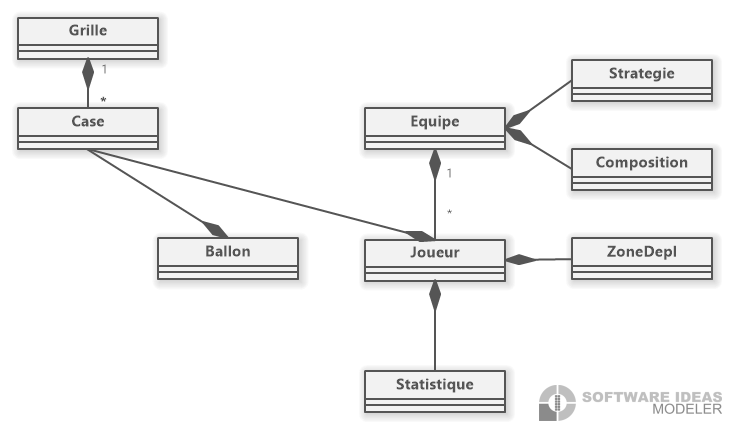
\includegraphics[width=17cm,height=15cm]{images/Classdiagram.png}
\caption{Classe de donnée}
\label{fig:classDonnee}
\end{figure}

\paragraph{}
    Comme on peut l'apercevoir sur \ref{fig:classDonnee}, une classe de donnée semble être la classe principale, c'est la classe Equipe. En effet, cela correspond a la réflexion que nous avons eux en début de projet, celle de se concentrer sur les blocs équipes avant de rentrer dans les réflexions individuelles.
\paragraph{}
    Aussi, a partir de \ref{fig:classDonnee}, on remarque la présence de statistiques unique a chaque joueur, le fait que les positions soient gérer par une grille et enfin la gestion des joueurs, de la stratégie et la composition est donnée à la classe Equipe.
    

\subsubsection{Systèmes de Manager}
\label{sec:managers}

\paragraph{}
    Dans cette section, nous détaillerons les différentes idées de conception autour de la gestion d'action et de déplacements.

\begin{table}[h!]
    \centering
    \begin{tabular}{|c|c|}
    \hline
    Nom Classe & Fonction\\
    \hline
    ManagBall & Gestion de toutes les actions autour du ballon\\
    \hline
    ManagDepl & Gestion de tous les deplacements de notre simulation\\
    \hline
    Manager & Classe qui permet la transmission et l'interaction entre les deux managers\\
    \hline
    \end{tabular}
    \caption{Répartition des taches entre les managers}
    \label{tab:managers}
\end{table}

\paragraph{Gestion des actions: }
    Comme expliquer dans \ref{tab:managers},la gestion des actions a été regrouper dans une seule et même classe : ManagBall. A l'intérieur de cette classe, les actions sont créer et peuvent interagir entre elles, par exemple, la possibilités de pouvoir intercepter la balle pendant une passe. C'est pour cela que nous avions décider de bien séparer la gestion des actions.

\paragraph{Gestion des déplacements: }
    Comme expliquer dans \ref{tab:managers},la gestion des deplacements a été regrouper dans une seule et même classe : ManagDepl. Comme expliquer dans \ref{sec:donnee}, la réflexion de toute la simulation est en priorité porter à l'équipe. Lors de la conception, nous avons imaginer le fonctionnement des déplacements de tel sorte que, d'abord, le bloc équipe monte ou descende en fonction de la possession ou non du ballon, puis seulement, un mouvement individuel des joueurs.
\newpage
\subsection{Conception IHM Graphique}
\label{sec:conceptGraph}

\paragraph{}
    Cette sous-section est dédiée aux ébauches d'idées de conception concernant toute la partie graphique du projet.
    
\begin{figure}[h]
\centering
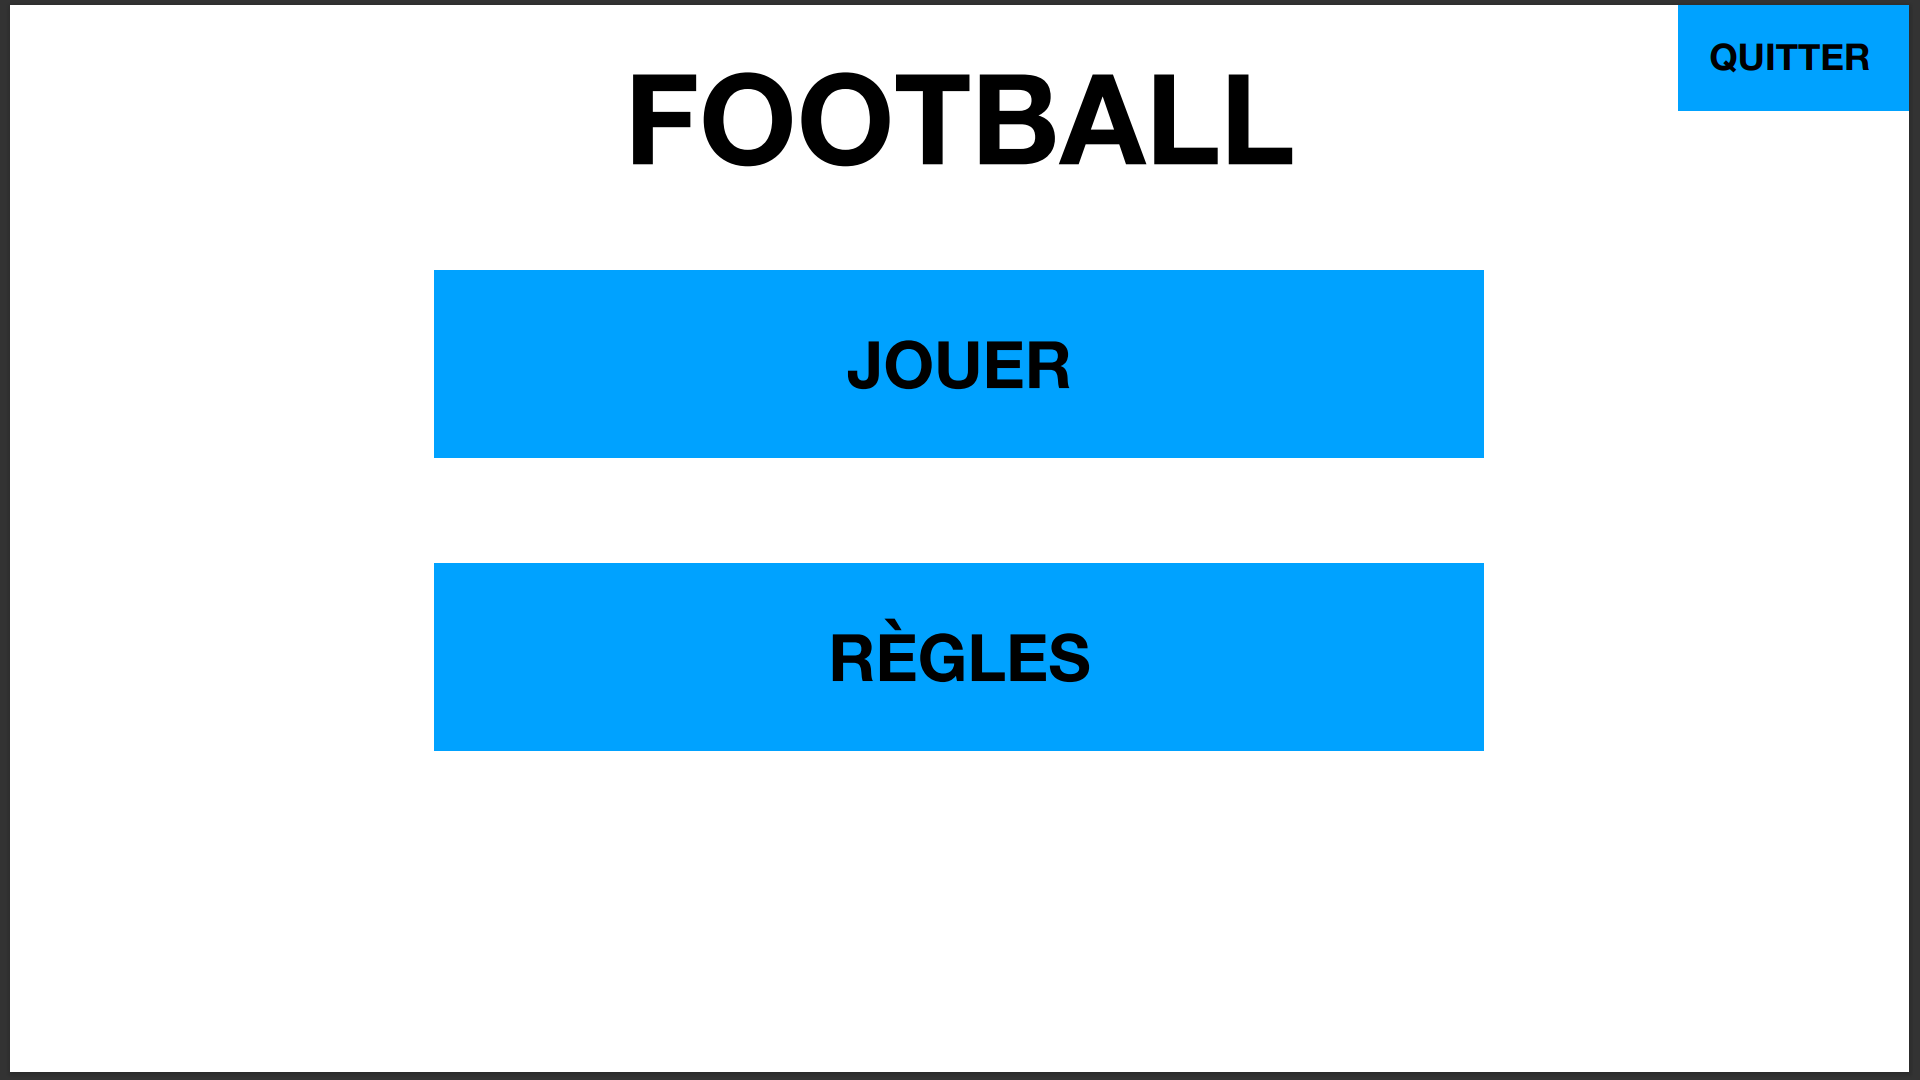
\includegraphics[width=12.82cm, height=8.2cm]{images/ConceptIHM1.png}
\caption{Conception page d'accueil}
\label{fig:accueil}
\end{figure}

\paragraph{Conception de la page d'accueil}
    Pour notre page d'entrée, notre première idée était de concevoir une page d'accueil basique que l'on peut voir dans n'importe quel jeu vidéo. 
    
    \vspace{15pt}

\begin{itemize}
    \item \textbf{Jouer :} 
        Si vous appuyez sur le bouton "Jouer" situé en haut, vous serez redirigé vers la page suivante qui vous permettra de choisir votre équipe.

    \vspace{15pt}

    \item \textbf{Règles :} 
        Si vous appuyez sur le bouton "Règles" situé au milieu, cela vous amènera sur la page des règles du jeu de football.

    \vspace{15pt}

    \item \textbf{Quitter :} 
        Si vous appuyez sur le bouton "Quitter" situé en bas, cela vous permettra de quitter le jeu.
        
    \vspace{15pt}
\end{itemize}

\newpage

\begin{figure}[h]
\centering
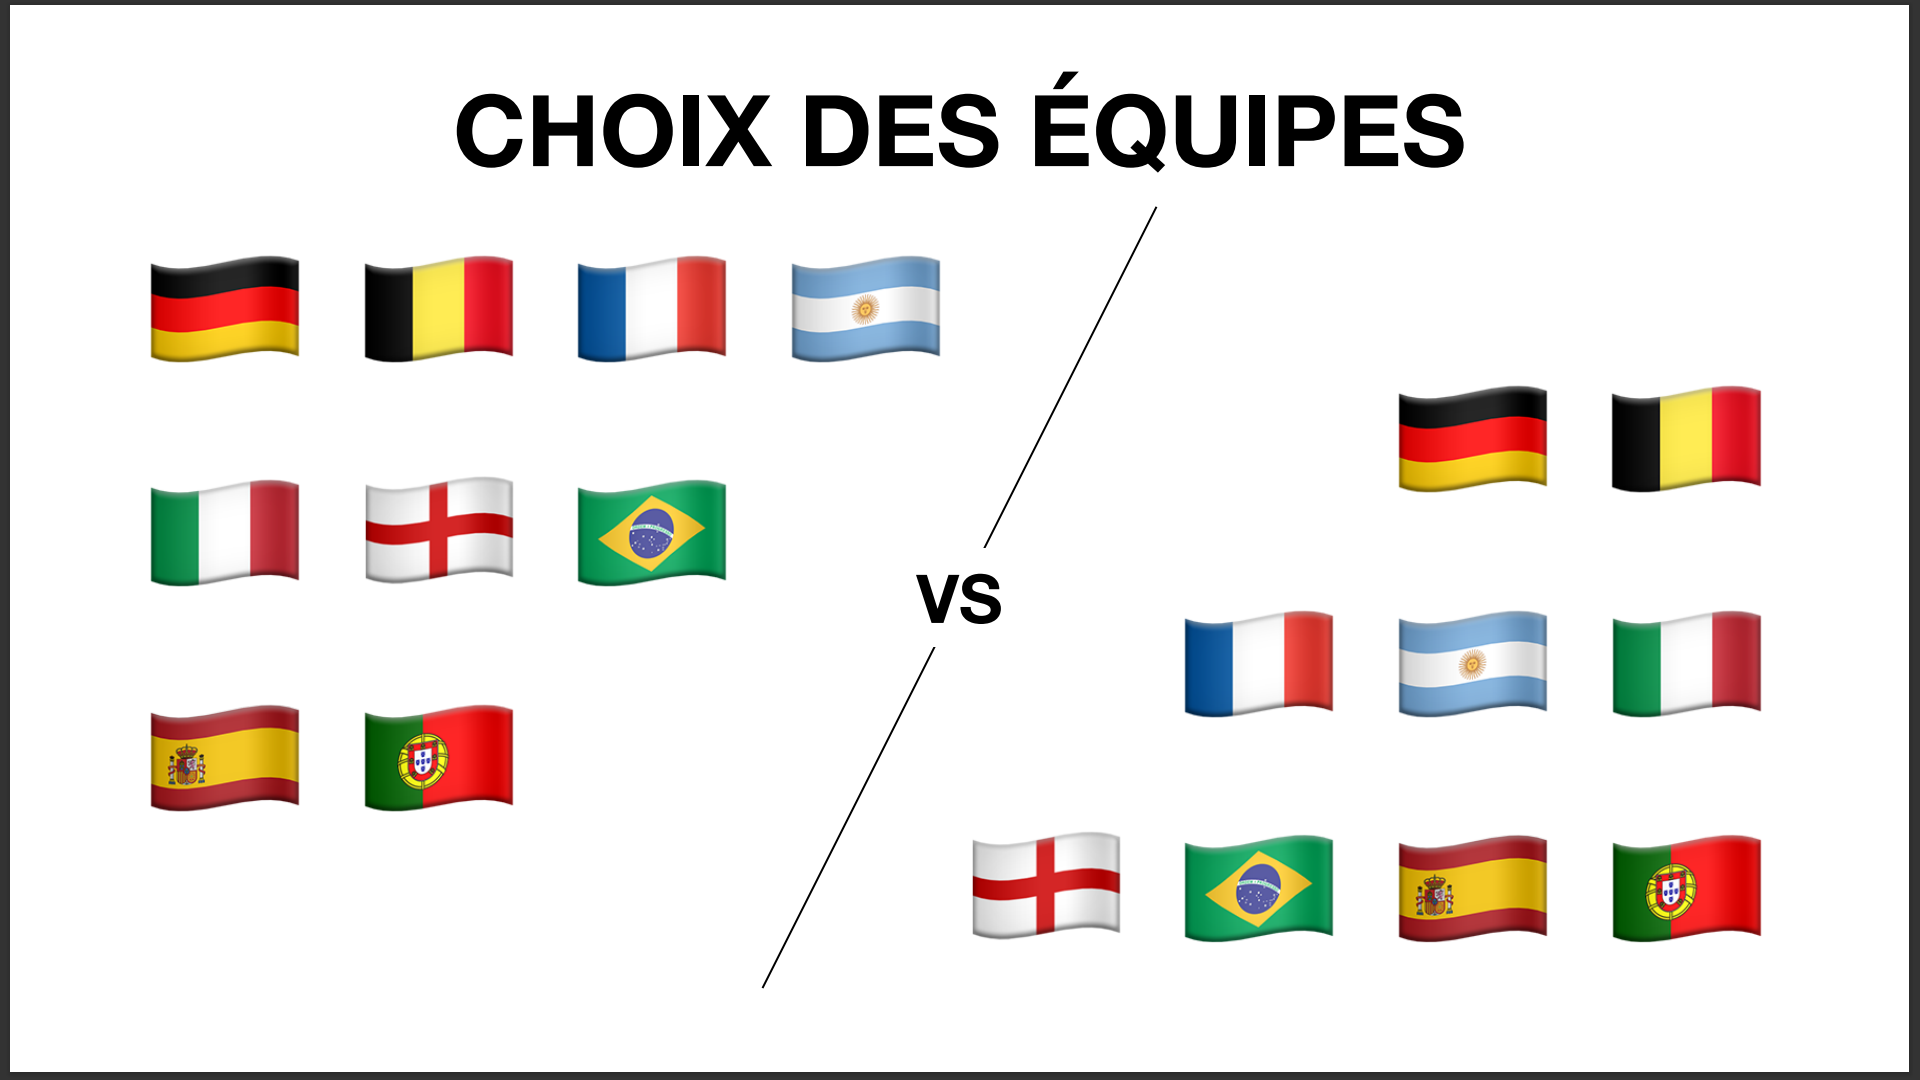
\includegraphics[width=12.82cm, height=8.2cm]{images/ConceptIHM2.png}
\caption{Conception Choix Equipe}
\label{fig:choixEquipe}
\end{figure}

\paragraph{Conception de la page du choix des équipes}
    On avait pour concept de permettre aux utilisateurs de choisir le pays que leur équipe représentera afin de leur donner le sentiment de maîtriser leur équipe et de leur permettre de choisir leur adversaire avant le match. Cette page est accessible depuis la page d'accueil lorsque le joueur clique sur le bouton "Jouer".

\vspace{15pt}
    
\begin{itemize}
    \item \textbf{Les équipes :} 
        Au milieu de l'écran, vous pouvez voir des drapeaux de pays parmi lesquels l'utilisateur pourra choisir celui qui représentera son équipe ainsi que celui de l'équipe adverse.
        
    \vspace{15pt}
\end{itemize}

\begin{figure}[h]
\centering
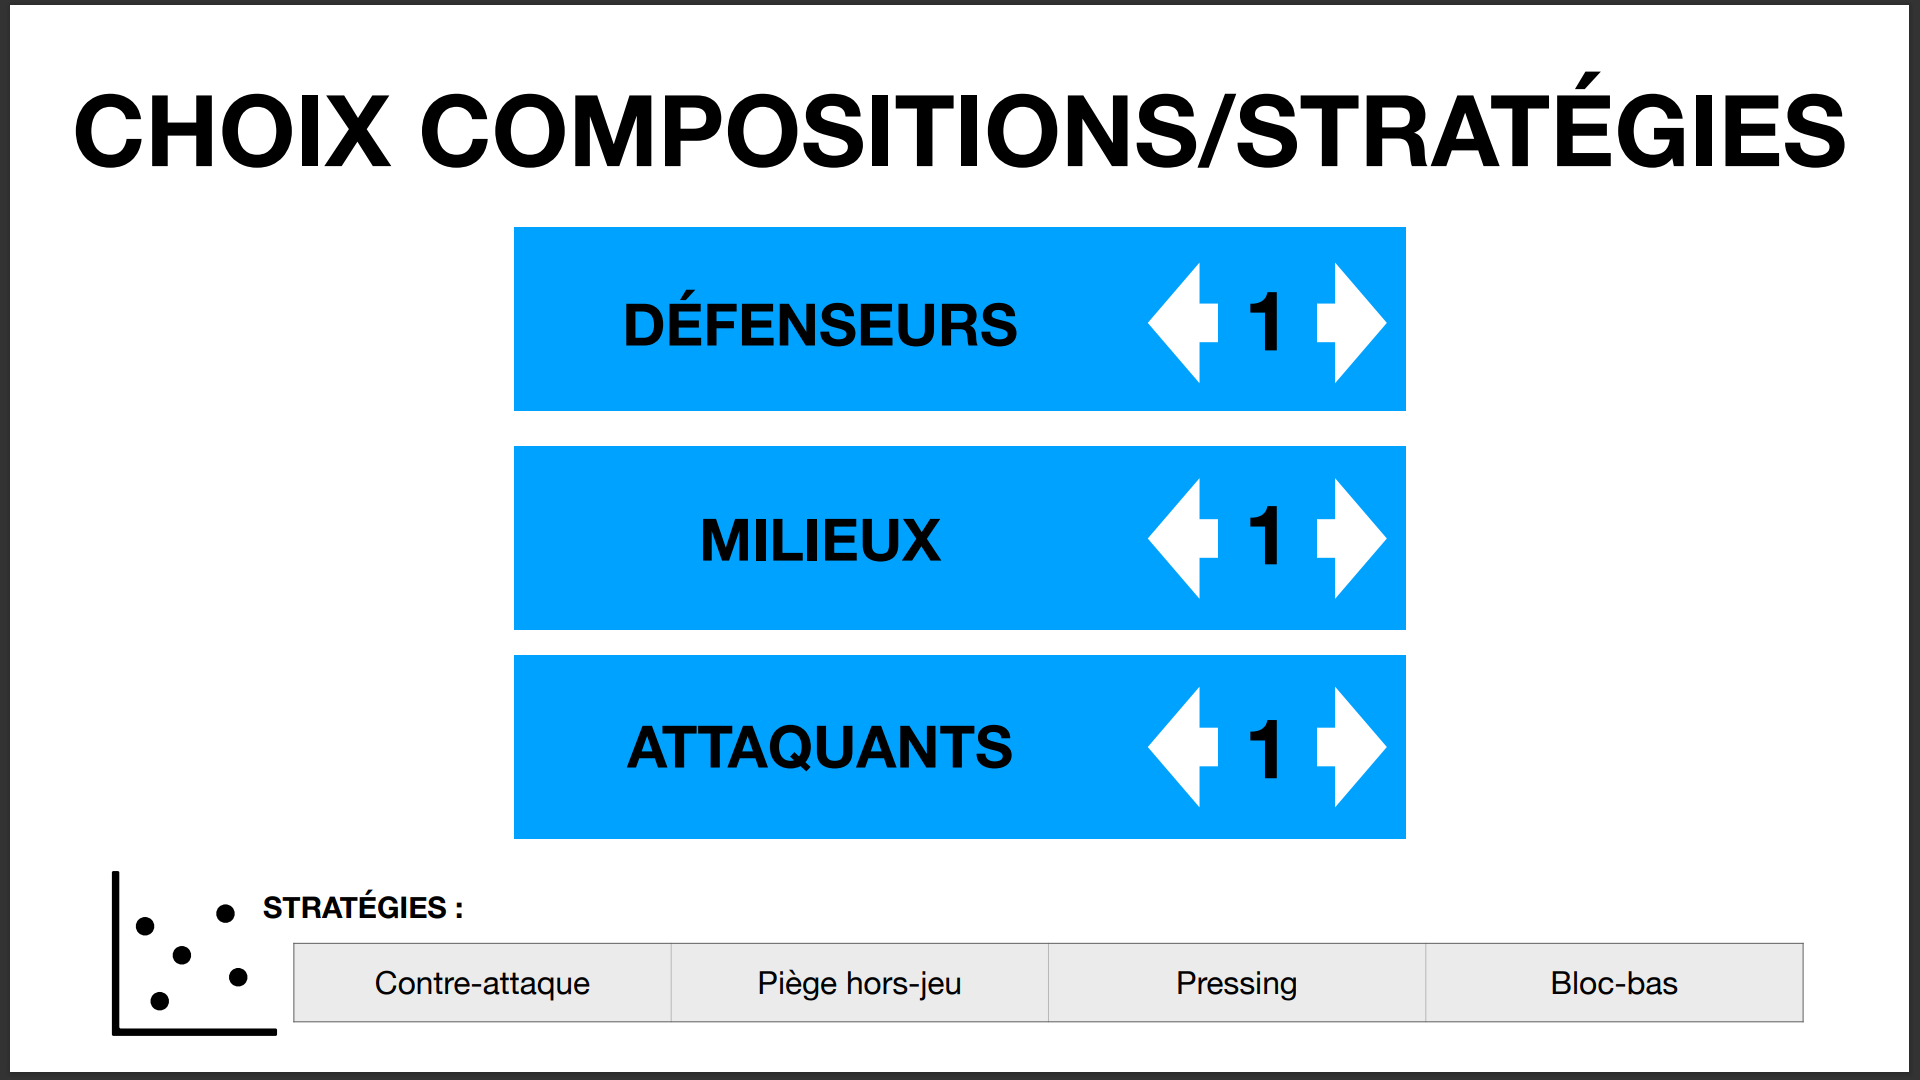
\includegraphics[width=12.82cm, height=8.2cm]{images/ConceptIHM3.png}
\caption{Conception Choix Poste}
\label{fig:choixPoste}
\end{figure}

    \vspace{15pt}
    \vspace{15pt}

\paragraph{Conception de la page de la sélection de votre composition}
    Cette page est l'une des plus importantes, car elle permet à l'utilisateur de choisir la composition de son équipe. Nous tenions vraiment à ce que l'utilisateur se sente maître de son équipe, c'est pourquoi nous lui donnons la possibilité de choisir sa formation. En ce qui concerne la stratégie, nous avons décidé de l'enlever, car nous avons jugé que son développement algorithmique serait trop compliqué à réaliser dans le temps imparti. Cette page fait suite à la page Choix des Équipes.

    \vspace{15pt}

\begin{itemize}
    \item \textbf{Les postes :} 
        Au milieu de votre écran, vous pouvez voir les différents postes avec deux flèches une vers la droite et l'autre vers la gauche, ainsi qu'un chiffre au milieu qui indique le nombre de joueurs sur chaque poste. Les flèches permettent d'ajouter ou de retirer un joueur à chaque poste.
    \vspace{15pt}
\end{itemize}

\begin{figure}[h]
\centering
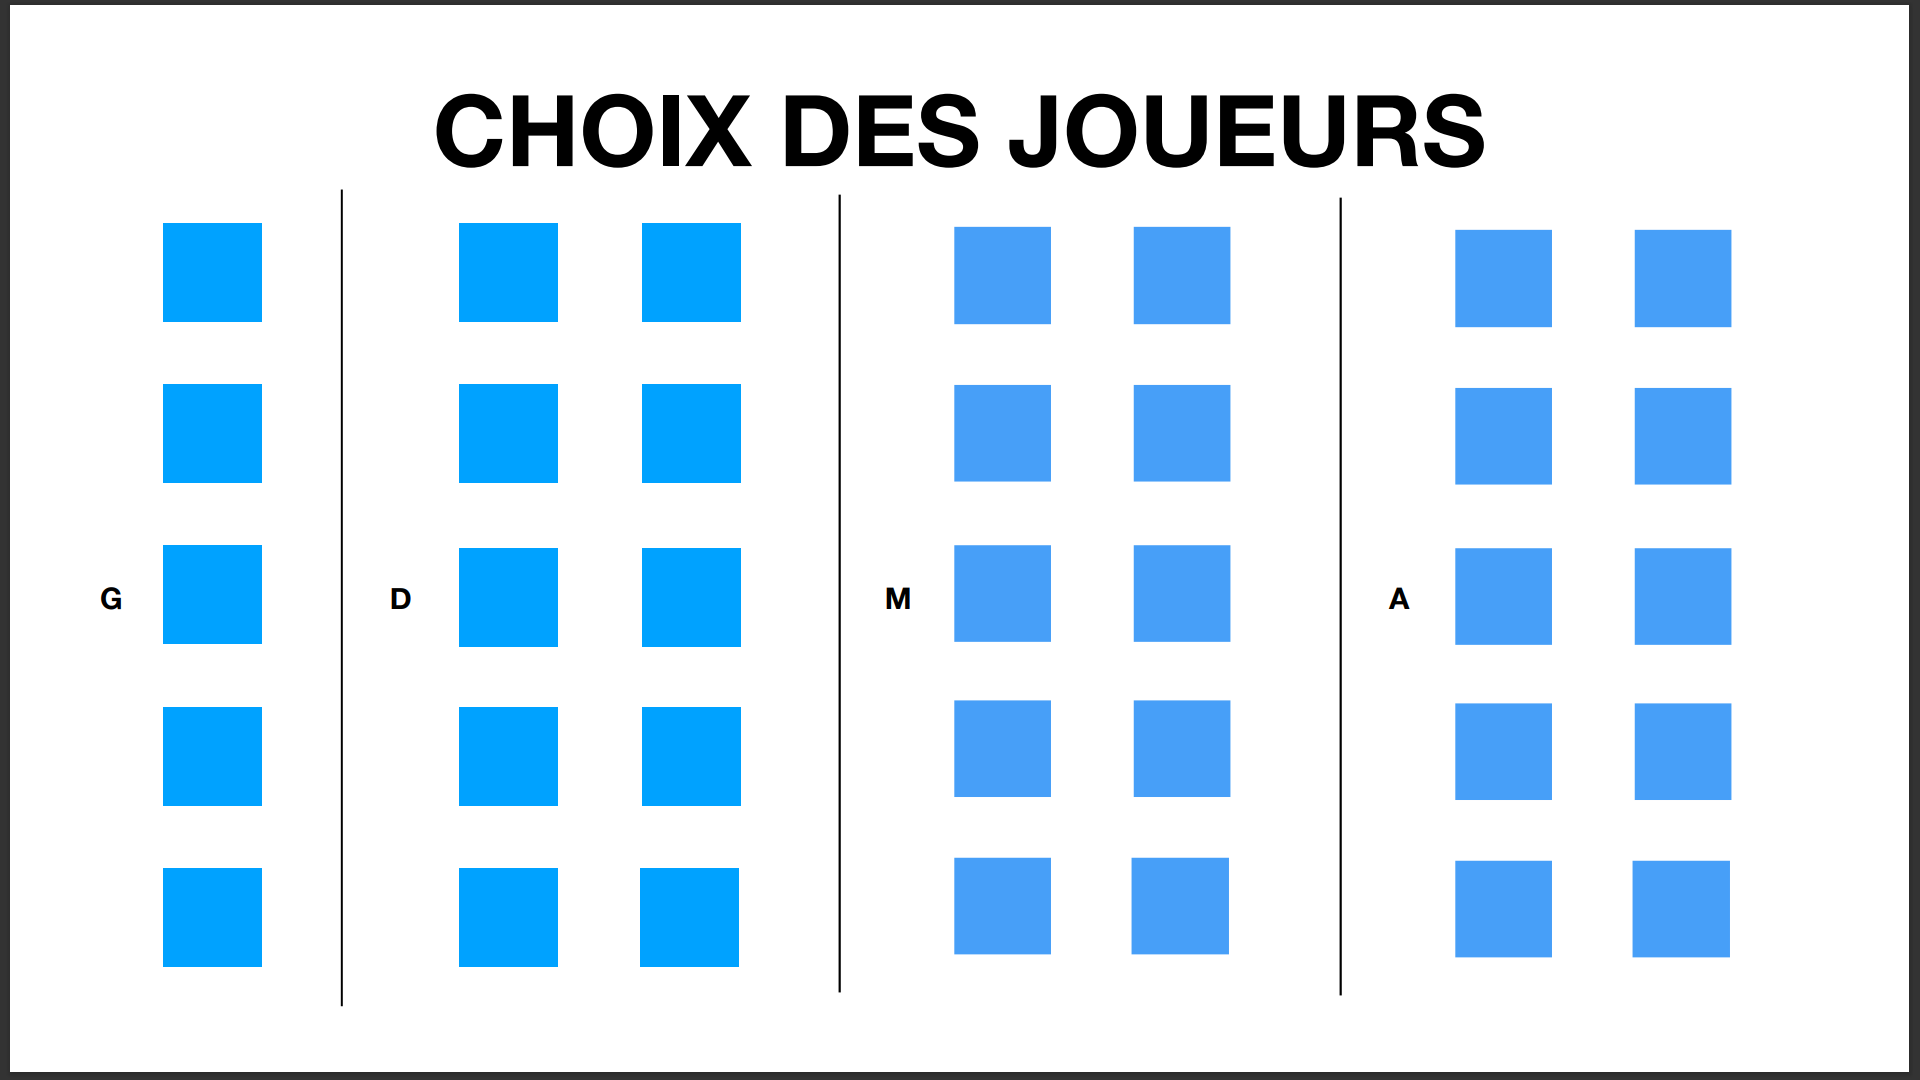
\includegraphics[width=12.82cm, height=8.2cm]{images/ConceptIHM4.png}
\caption{Conception Choix Joueur}
\label{fig:choixJoueur}
\end{figure}

    \vspace{15pt}

\paragraph{Conception de la page de la sélection de vos joueurs}
    Cette page est l'une des pages les plus importantes puisque elle permet à l'utilisateur de choisir les joueurs qui composeront son équipe. Nous avons décidé de laisser à l'utilisateur la possibilité de choisir les joueurs pour qu'il puisse prendre les meilleurs joueurs disponibles et ainsi être le chef d'orchestre de son équipe. Cette page fait suite à la page Choix de Postes.

    \vspace{15pt}

\begin{itemize}
    \item \textbf{Les joueurs :} 
         Au milieu de l'écran, l'utilisateur peut sélectionner les joueurs pour chaque poste en cliquant sur le chiffre correspondant. Par exemple, s'il a choisi d'avoir trois attaquants dans la page précédente, il peut sélectionner 3 attaquants en cliquant sur les joueurs à côté de "A". Il peut faire de même pour le gardien "G", les défenseurs "D" et les milieux "M".
    \vspace{15pt}
\end{itemize}

\newpage

\begin{figure}[h]
\centering
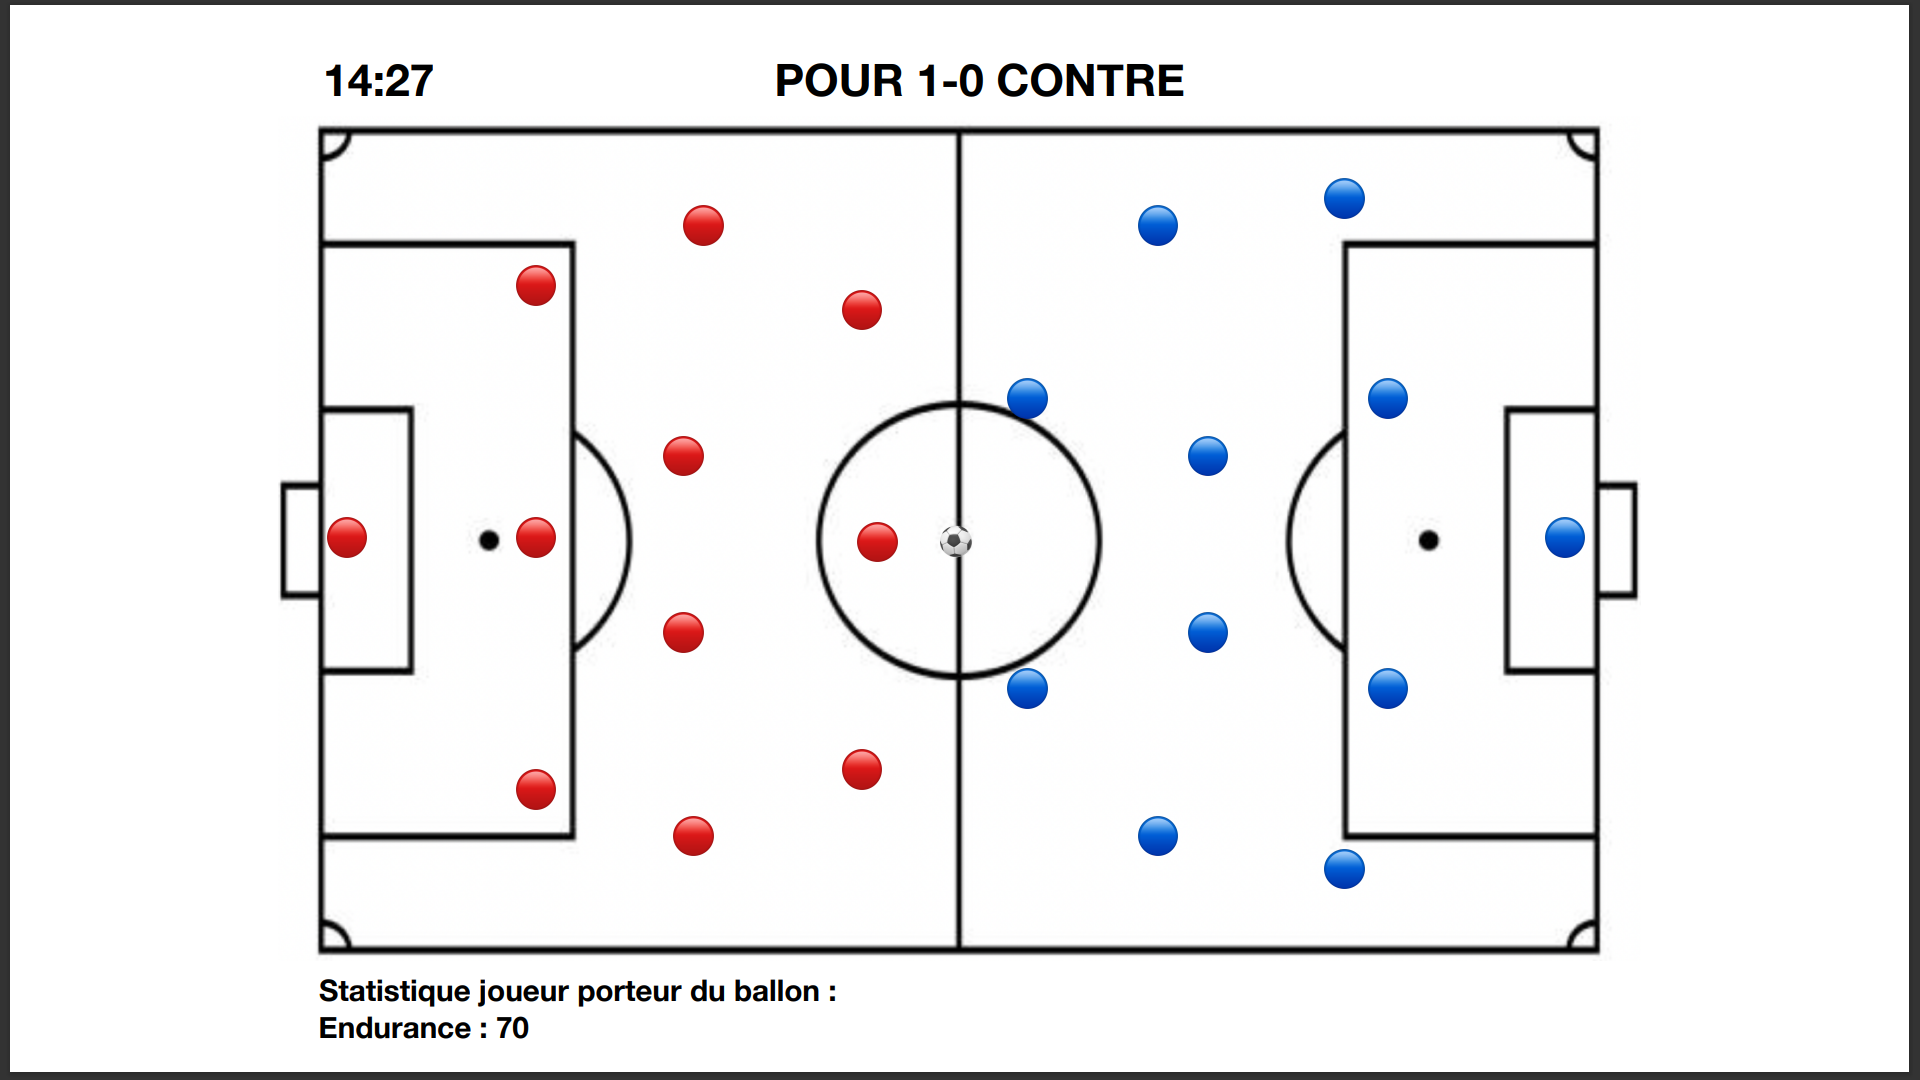
\includegraphics[width=12.82cm, height=8.2cm]{images/ConceptIHM5.png}
\caption{Conception de la simulation }
\label{fig:match}
\end{figure}

    \vspace{15pt}
\paragraph{Conception de la page de la simulation du match}
    C'est la page principale de notre simulation, car c'est lors du match que tous les choix de l'utilisateur vont s'impliquer. Nous avons voulu rester fidèles à l'expérience d'un match de football en permettant à l'utilisateur de voir le score et le temps. Nous avons décidé de ne pas afficher le joueur ayant la balle, car nous ne l'avons pas jugé pertinent. Cette page est la suite de la page Choix des Joueurs.

\vspace{15pt}

\begin{itemize}
    \item \textbf{Temps :} 
        Le chronomètre est indiqué à gauche des scores pour vous permettre de savoir combien de temps il reste avant la fin du match.

    \vspace{15pt}

    \item \textbf{Score :} 
         Le score est affiché juste au dessus du terrain. Ainsi, si l'équipe de l'utilisateur marque, il pourra le voir directement à cet endroit.

    \vspace{15pt}
            
    \item \textbf{Statistique du joueur ayant la balle :}
        La base de notre idée était de permettre à l'utilisateur de voir les statistiques du joueur ayant la balle en dessous du terrain, mais nous avons décidé de l'enlever comme cela a été expliqué précédemment.
    
    \vspace{15pt}
\end{itemize}

\newpage

\begin{figure}[h]
\centering
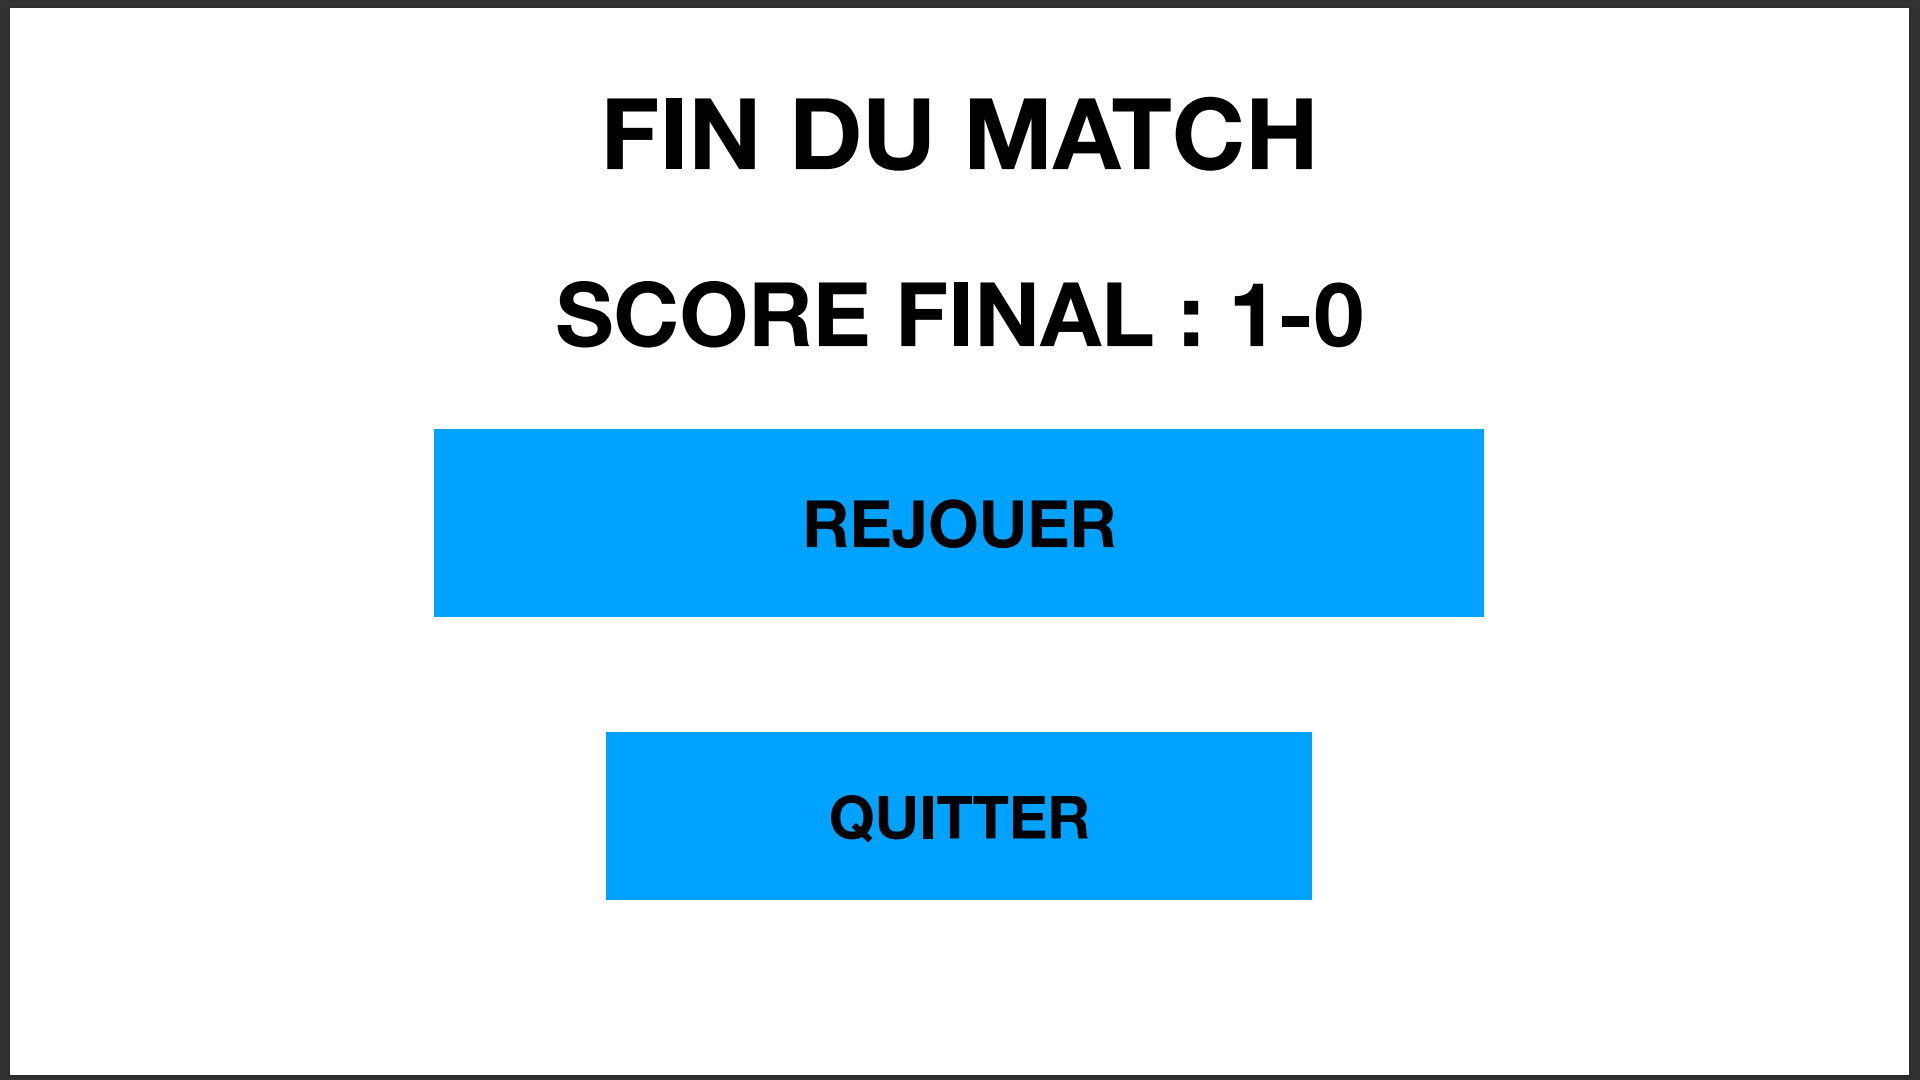
\includegraphics[width=12.82cm, height=8.2cm]{images/ConceptIHM6.png}
\caption{Conception Après Match}
\label{fig:stats}
\end{figure}

\vspace{15pt}

\paragraph{Conception de la page d'après match}
    Cette page est la dernière page après avoir fini le match. Elle permet la redirection vers la page d'entrée.

\vspace{15pt}
    
\begin{itemize}
    \item \textbf{Rejouer :} 
        Si vous appuyez sur le bouton "Rejouer", vous serez redirigé directement vers la page du choix des équipes.

    \vspace{15pt}

    \item \textbf{Quitter} 
         Si vous appuyez sur le bouton "Quitter", cela vous fera quitter la simulation.

    \vspace{15pt}
            
    \item \textbf{Le score :}
        Le score situé au-dessus du bouton "Rejouer" est le score de fin de match.
        
    \vspace{15pt}
\end{itemize}
\newpage
\section{Réalisation du projet}
\label{sec:realisation}

\noindent Cette section fait écho à la section précédente \ref{sec:concept}. Ici, nous détaillerons la mise en oeuvre effective de notre conception.

\subsection{Solution moteur}

\paragraph{}
    Dans cette sous-section, nous décrirons en détail les solutions mises en place pour le gestion algorithmique du logiciel.

\subsubsection{Point de vue global}

\paragraph{}
    Il est important de préciser le fonctionnement globale de notre noyau pour bien comprendre les solutions moteurs utilisaient et leurs différents appels.

\paragraph{}  
    Notre simulation fonctionne sur une boucle principale avec notre Thread qui fait appel a chaque itération a la méthode advance de Manager. C'est a partir de la que les actions ou les déplacements seront gérés a partir d'ici par les différents managers.

\paragraph{}
    Ensuite, c'est boucle principale va être limiter dans le temps par un chronomètre qui va être incrémenter et allant jusqu'à 90 : 00, temps a partir duquel le jeu s'arrête.


\subsubsection{Système d'action}

\paragraph{}
    Ici, nous détaillerons les solutions apportées dans la classe ManagBall pour gérer les actions lors de la simulations. Nous considérons comme action, toutes interactions de joueur avec le ballon.

\paragraph{Choix d'action}
    D'abord, il serait intéressants de préciser comment est réalisé le choix d'une action. A l'intérieur de la classe, il y a un attribut qui permet le stockage des actions a réaliser, une ArrayList contenant des objet de type Action qui correspond a notre Interface pour toute nos actions. Lorsque cette attribut est vide, il faut choisir une action adapte, pour cela nous récupérons le Joueur en possession du ballon puis a partir d'un nombre important d'information, nous calculons deux scores. Premièrement, un score pour le choix d'un tir : ce score prend en compte l'avancement du joueur par rapport au but adverse, la distance par rapport au joueur adverse le plus proche, si la zone de déclenchement du tir est acceptable et enfin si le joueur est seul face au gardien. Ensuite, si le score est suffisamment haut, l'action Tir est crée et ajouter à la liste d'actions. Cependant si le score n'est pas suffisant, viens alors le calcul d'un deuxième score pour la réception d'une passe qui permet de choisir le meilleur receveur possible pour la passe qui est ensuite crée et ajoutée dans la liste.

\paragraph{}
    Évidemment, les Passe et les Tir ne sont pas les seules actions de notre simulation. Cependant les autres actions découlent directement de ces deux là. En effet, pour l'action Arrêt, l'action ne peut être tenter qu'une seule fois par Tir et en fonction de la statistique d'Arret du gardien peut amener a une corner. Pour l'action Interception, elles sont créer lorsqu'une action se situe déjà dans la liste et a chaque passage chaque joueur adverse aura la possibilité d'intercepter la balle. Les chances d'interception dépendent de la distance avec le ballon et de la statistique de défense du joueur.

\paragraph{}
    Enfin, la possibilité d'action spéciale tel que les fautes, les corners, les hors-jeux ou encore les sorties de but fonctionnent d'une manière différente qui n'utilise pas la liste d'action mais par une système d'exception pour permette la transmission d'informations nécessaires et des changements aux autres managers.

\paragraph{Réalisation des actions}
    Une fois la création des actions faites, il faut maintenant les réaliser et, durant cette réalisation, il y a plusieurs aspect intéressant tels que le calcul des trajectoires du ballon pour les passes ou les tirs, l'utilisation du visiteur pour réaliser les actions sans se soucier du type précis de l'action de la même famille qui implémente Action ou encore le système d'exception pour la remonter d'information.

\begin{equation}
coef = ((LigneAct - LigneCible)*10)/(ColonneAct - ColonneCible)
\label{eq:coeff}
\end{equation}

\paragraph{}
    Pour comprendre le calcul des trajectoires, il faut voir la formule \ref{eq:coeff} pour le coefficient qui détermine les déplacements a réaliser pour arriver a atteindre la cible donnée. En fonction du résultat de notre coefficient, on va déplacer l'objet (ici le ballon) d'un nombre de case un ligne et/ou colonne obtenu par des calculs sur le coefficient. Ce calcul de trajectoire est utiliser pour les tirs où la cible est une Case sur la colonne des cages adverse mais où la ligne est choisi parmi une plage de case centre autour des cages qui se réduit en fonction de la statistiques de Tir du tireur. Quand le calcul de trajectoire est réaliser pour une passe, la trajectoire suit la position du joueur pendant le déplacement de celle-ci. Le calcul de trajectoire est situe dans la classe Utility.

\paragraph{}
    Maintenant, nous allons détailler l'utilisation d'un pattern Visitor pour la réalisation des actions. Et pour pouvoir utiliser ce pattern, toutes les actions ont été regroupées dans une famille de classe qui implémente l'interface Action qui oblige l'implémentassions d'une méthode visit pour le passage d'un visiteur.

\paragraph{}
    D'abord, nous avons décider d'utiliser ce pattern Visitor car il nous permet de bien gérer les différentes actions de manière singulière sans surcharger le code de ManagBall et aussi de gérer le retour pour permettre une vérification simple de la fin d'une action. En effet, pour réaliser cela, nous avons créer un visiteur RealActionVisitor avec pour type de retour Boolean qui retourne vrai quand l'action est terminée ce qui permet lors du parcours de la liste d'action de la supprimer de cette liste (voir algorithme \ref{algo:visit})

\begin{algorithm}
\caption{Fonction parcourant liste des actions}
\label{algo:visit}
\begin{algorithmic} 
\STATE $iter \leftarrow array.iterator$
\WHILE{$iter.hasNext()$}
\STATE $ act \leftarrow itr.next()$
\IF{$act.accept(real)$}
\STATE $itr.remove()$
\ENDIF
\ENDWHILE
\end{algorithmic}
\end{algorithm}

\paragraph{}
    Ensuite, à l'intérieur de RealActionVisitor, on décrit tous les comportements relatifs a la réalisation des actions. Pour une passe, l'avancer du ballon vers la cible, de la même manière pour une tir. Pour un arrêt, a la manière d'un jets de dés dans un jeu de rôle, on récupère un entier aléatoire de 1 à 100 et si le score est inférieur ou égale a la statistique d'arrêt divisé par deux alors l'action est réussi puis on recommence pour savoir si la balle lui échappe et part en corner.Ce dernier exemple nous amène au dernier point intéressant de la réalisation d'action, l'utilisation d'exception pour les actions spéciales.

\paragraph{}
    En effet, les actions spéciales découlent directement de conditions spécifiques des actions normales. Et souvent, amène a des changement de possession ou des arrêt du jeu qui nécessite la communication avec les autres managers. Pour pouvoir réaliser cela, nous avons fait appelle aux exceptions. Du coup, lorsque les conditions sont réunies, le visiteur lève une exception qui va remonter jusqu'à la méthode principale de ManagBall calcul qui va traiter l'exception. Puis l'exception va ensuite remonter jusqu'à la classe Manager pour modifier la possession du ballon, gérer le replacement des deux équipes et aussi mettre pause au jeu puis reprendre la simulation.

\paragraph{Exemple}
    Pour finir, nous allons tracer ensemble les différents appels réaliser lors d'un Hors-jeu.
    
\paragraph{}
    D'abord, l'exception Hors-jeu a un comportement particulier. Juste avant la création de la passe, on vérifie si le joueur est en position de Hors-Jeu, si il est en position de Hors-jeu alors on change un booléen en vrai et on réalise la passe. Lorsque la passe a été réaliser, avant le choix d'une nouvelle action,on retire la possession du ballon a tous les joueurs de l'équipe, on change de possession dans ManagBall et on lève l'exception HorsJeuException.
    
\paragraph{}    
    Ensuite, l'exception arrive dans la classe Manager où elle est traité : d'abord, on mets la simulation en pause, on change la position dans ManagDepl et dans Manager, on précise que l'action de reprise sera de type coupFrancs avec la précision de l'attribut variable puis on récupère la position de l'hors-jeu stocke dans l'exception que l'on stocke dans un joueur créer spécifiquement pour l'occasion. Après, on mets en place la reprise du jeu avec le positionnement des joueurs et l'attribution de la balle. Enfin,la simulation reprend avec une liste d'action vide dans ManagBall.
    

\subsubsection{Système et calcul des déplacements}

\paragraph{}
    Le calcul des déplacements est réalisé selon les cases de notre terrain, ils en font des coordonnées que l'on utilise dans chaque méthode de déplacement. Aussi, les déplacements peuvent être diviser en deux catégories, le bloc équipe et les déplacements individuels

\paragraph{Bloc équipe}
    Dans un premier temps, les déplacement d'une équipe possédant le ballon sont réaliser de façon a se rapprocher le plus des cages de l'équipe adverse. Pour cela, il y aura d'abord un mouvement global des deux équipes (vers l'avant pour l'équipe ayant la possession et vers l'arrière quand ils n'ont pas la possession). Les joueurs seront limiter dans leur avancer par la vérification dans la classe Strategie de la position de la ligne des défenseurs. En effet, le bloc équipe arrêteras d'avancer lorsque les défenseurs atteindront la ligne médiane ce qui lancera la possibilité de déplacement individuel.
     

\paragraph{Deplacements Individuel}
    En ce qui concerne les deplacements individuels il y aura deux cas de figures : le cas ou l'equipe a le ballon et l'inverse. 

\paragraph{}
    Lorsque son equipe a la possession du ballon, les joueurs chercheront a aller de l'avant et à se démarquer en récupérant les coordonnées des joueurs de l'équipe adverse, et par ce fait, s'en écarter au maximum, tout en restant dans sa zone tactique. Il peut arriver qu'un joueur de l'équipe qui possède le ballon recule, seulement dans le cas ou il est marqué de trop près par joueur adverse, et ainsi il un déplacement vers l'arrière. Seul les milieux de terrains et les attaquants adoptent ces déplacement. Les défenseurs eux restent sur la ligne médiane du terrain, et le gardien reste dans ses buts.
    
\paragraph{}
    Dans un second temps, les déplacements des joueurs de l'équipe ne possédant pas le ballons, sont basés sur ceux des joueurs possédant le ballon. Leur but à eux sera de se rapprocher au maximum des milieux de terrains et des attaquants via un marquage individuel, afin d'avoir le plus de chance d'intercepter le ballon lorsqu'un joueur le reçoit, de par sa proximité qui augmente ses chances de récupérer le ballon. Ainsi, chaque milieux de terrain marqueront un milieu de terrain adverse, et chaque défenseurs marqueront un attaquant adverse. En ce qui concerne les attaquants, ils ne réalisent le marquages des défenseurs adverse seulement dans le cas où les défenseurs possède le ballon ou bien qu'ils en sont la cible : 
    
\begin{figure}[h]
\centering
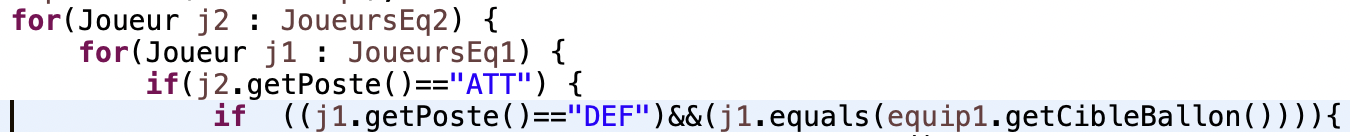
\includegraphics[width=15cm]{images/code_marquage.png}
\label{fig:marquage}
\end{figure}
       
\paragraph{}
    Avec le code \ref{fig:marquage}, les attaquants effectueront les déplacements vers les défenseurs uniquement en cas de possession de la balle d'un défenseur.

\paragraph{}
    Ensuite, lors d'un changement de possession de la balle, soit lors d'une interception par exemple, l'équipe dépossédée du ballon va se repositionner en bloc, via l'appel d'une méthode permettant le replacement d'un joueur dans sa zone tactique, déterminée par la composition choisie au préalable. En parallèle de ça, le bloc redescendra sur le terrain, afin de se repositionner de façon défensive. Et vice versa, l'équipe qui récupère le ballon elle, va monter sur le terrain afin de se mettre en position offensive, en bloc haut.
\paragraph{D2placement Gardien}
       En ce qui concerne les déplacements des gardiens, ils sont les mêmes pour les deux gardiens. Lorsque le ballon arrive a une certaine distance des buts, le gardien se positionnera dans l'axe du ballon afin d'être suffisamment bien placé lors d'un tir.

\begin{figure}[h]
\centering
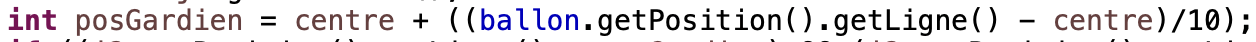
\includegraphics[width=15cm]{images/code_posgardien.png}
\label{fig:posGardien}
\end{figure}

\paragraph{}
   De plus, lorsque le ballon est situé dans une zone de 20 cases devant les buts, le gardien s'alignera avec la balle, en essayant de se mettre sur la même case que cette dernière afin de maximiser ses chances de l'arrêter.
\begin{figure}[h]
\centering
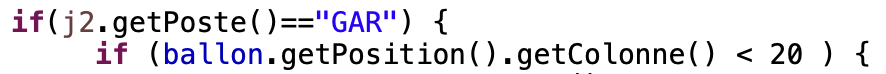
\includegraphics[width=10cm]{images/code_gardien.png}
\label{fig:gardien}
\end{figure}

\paragraph{Cas Particulier}
    Il existe un cas particulier lors de l'apparition de certaines actions spéciales. Le  cas du replacement du joueur qui réalise un corner ou une sortie de but.

\paragraph{}
    En effet, lorsqu'un joueur réalise ce genre d'action, il n'est plus positionné dans sa zone tactique, zone dans laquelle il réalise des déplacement. De ce fait, lors de l'arrivée de tel cas dans Manager, on récupère le joueur dans une variable centreur puis on l'oblige a se déplacer jusqu'à sa zone tactique ce qui empêche le joueur de rester bloque à l'endroit de son action jusqu'au prochain changement de possession.
    
\subsection{Solution IHM Graphique}

\paragraph{}
    On regroupera ici les solutions implémentées intéressante pour l'interface graphique du logiciel, selon les conceptions énoncés dans la section \ref{sec:conceptGraph}.

\paragraph{Choix Joueurs}
    Une des solutions intéressantes de notre IHM Graphique me semble être notre façon de gérer la sélection des Joueurs.

\paragraph{}
    La solution que l'on a implémenter diffère de notre conception, en effet, la sélection ne se fait plus dans la même fenêtre mais dans une fenêtre pour chaque poste. Et pour accéder aux différents postes, cela va se faire en fonction du constructeur choisi en fonction du nombre d'ArrayList donne en paramètre qui représentent les postes où les joueurs ont déjà étés sélectionnés.
    
\paragraph{}
    Ensuite, une fois le poste à remplir déterminer, pour que la sélection des joueurs soit visuel, il y a l'apparition des joueurs générer dans un JPanel à gauche sous forme de JLabel puis avec un MouseListener qui agit sur les JLabel, on les transfert sur le JPanel des Joueurs sélectionner à droite tout en vérifiant que l'on ne dépasse pas le nombre de joueur donner par le composition de l'équipe définit précédemment par l'utilisateur.

\paragraph{Statistique}
    Un autre élément important de notre IHM Graphique est la gestion et générations des statistiques. Pour décrire cela, on va d'abord détailler la récolte des informations puis la génération et l'affichage des graphiques.
    
\paragraph{}
    Pour la récolte des données, on récupère deux données. D'abord, lors de la création du terrain et l'affichage du match, on visite tous les joueurs des deux équipes pour calculer la moyenne de toutes les statistiques des joueurs puis dans ChartManager on génère un histogramme grâce à JFreeChart puis on le retourne dans un ChartPanel pour l'afficher sur l'écran. Ensuite, la seconde récolte de donnée se situe dans Manager pour récupérer toutes les occurrences des actions réalisé pendant le match. Ces informations seront exploitées lors de l'écran final de notre jeu comme un comparatif des actions réalise par les deux équipes.
    
\newpage
\section{Manuel utilisateur}
\label{sec:manuel}

\noindent Cette section est dédiée au manuel utilisateur. Ici, nous allons détailler les différentes actions, données dans \ref{sec:spec2} et \ref{sec:realisation}, sous la forme d'un guide pour l'utilisateur.

\subsection{Avant le match}

\paragraph{}
    Dans cette sous-section, nous allons détailler les différents écrans possible avant le match, avec des captures d'écrans légendes, pour expliquer les différentes actions possibles à l'utilisateur.

\begin{figure}[h]
\centering
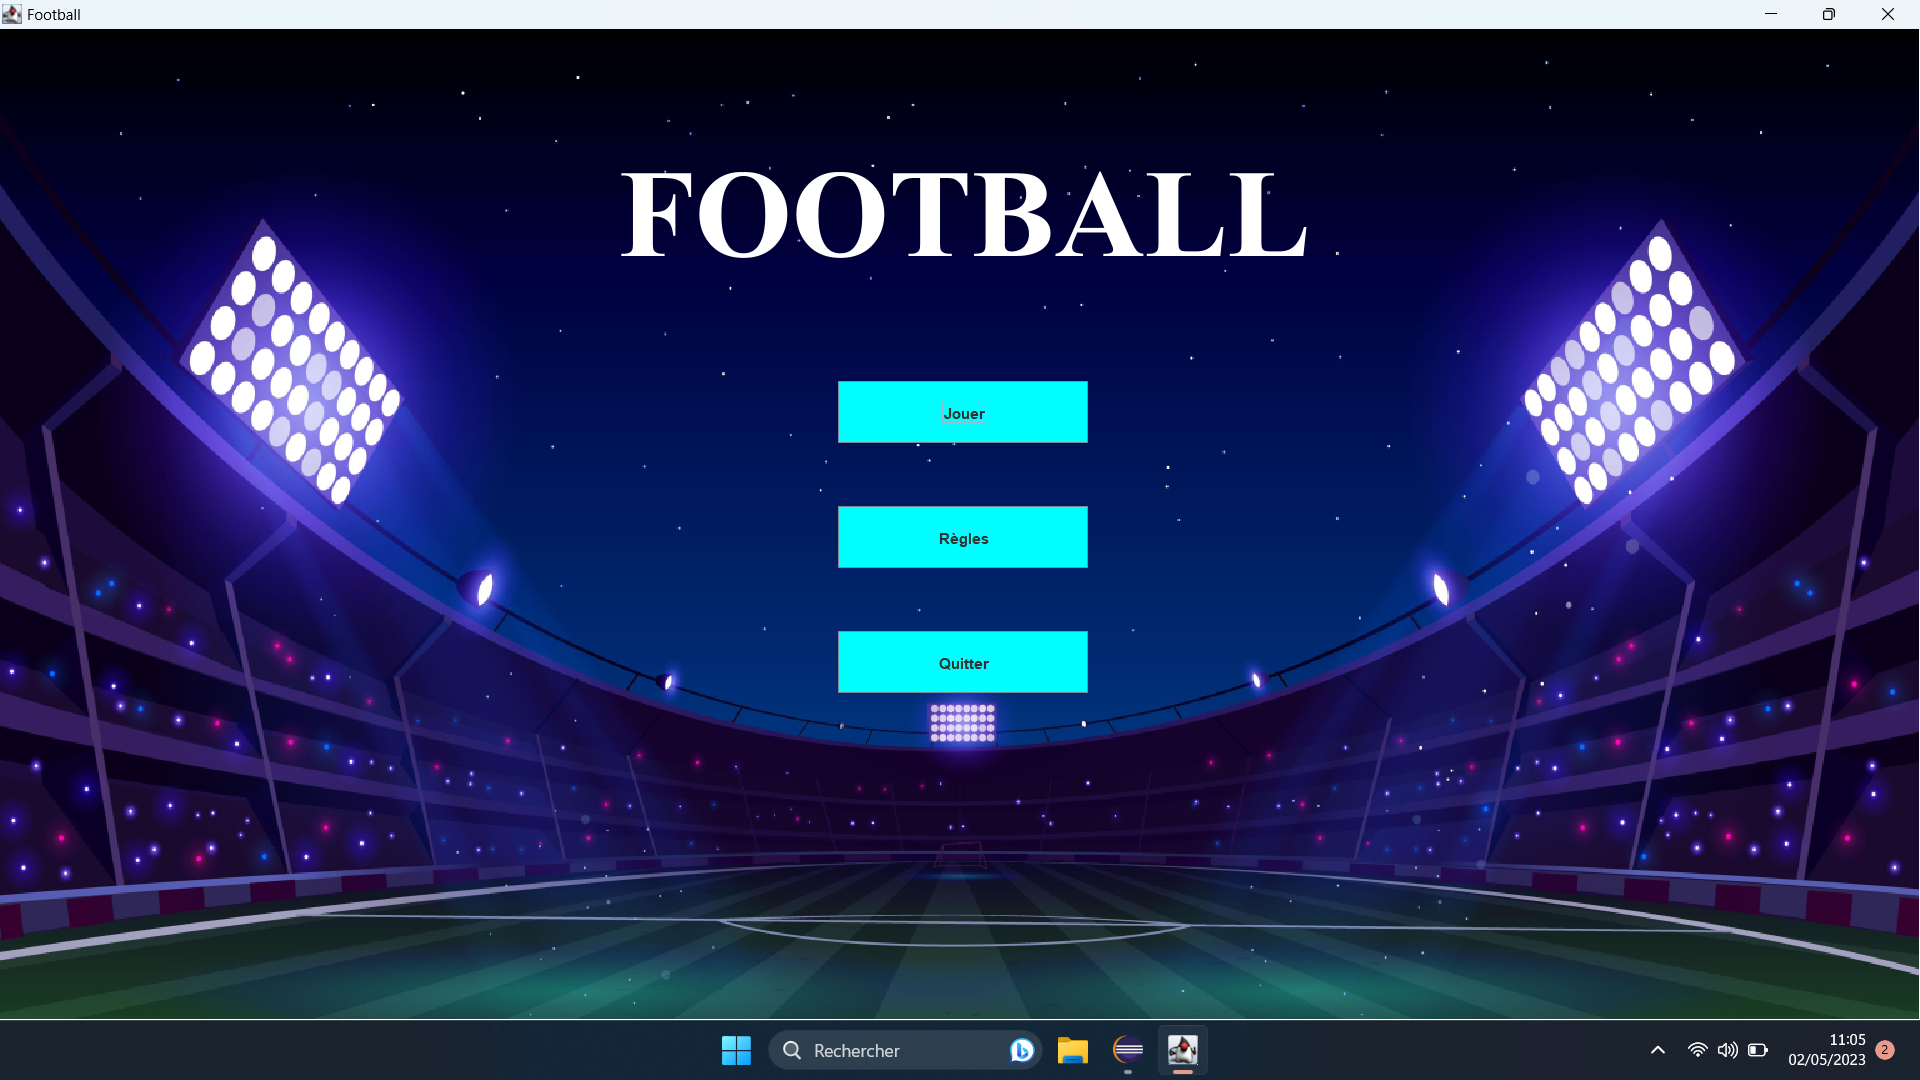
\includegraphics[width=12.82cm, height=8.2cm]{images/Accueil.png}
\caption{Page d'accueil}
\label{fig:accueil}
\end{figure}

\paragraph{Page d'accueil}


\begin{itemize}
    \item \textbf{Jouer :} 
        Si vous appuyez sur le bouton "Jouer" situé en haut, cela vous amènera à la page suivante qui est le choix d'équipe.

    \vspace{15pt}

    \item \textbf{Règles :} 
        Si vous appuyez sur le bouton "Règles" situé au milieu, cela vous amènera sur la page des règles du football.

    \vspace{15pt}

    \item \textbf{Quitter :} 
        Si vous appuyez sur le bouton "Quitter" situé en bas, cela vous fera quitter le jeu.
        
    \vspace{15pt}
\end{itemize}

\newpage

\begin{figure}[h]
\centering
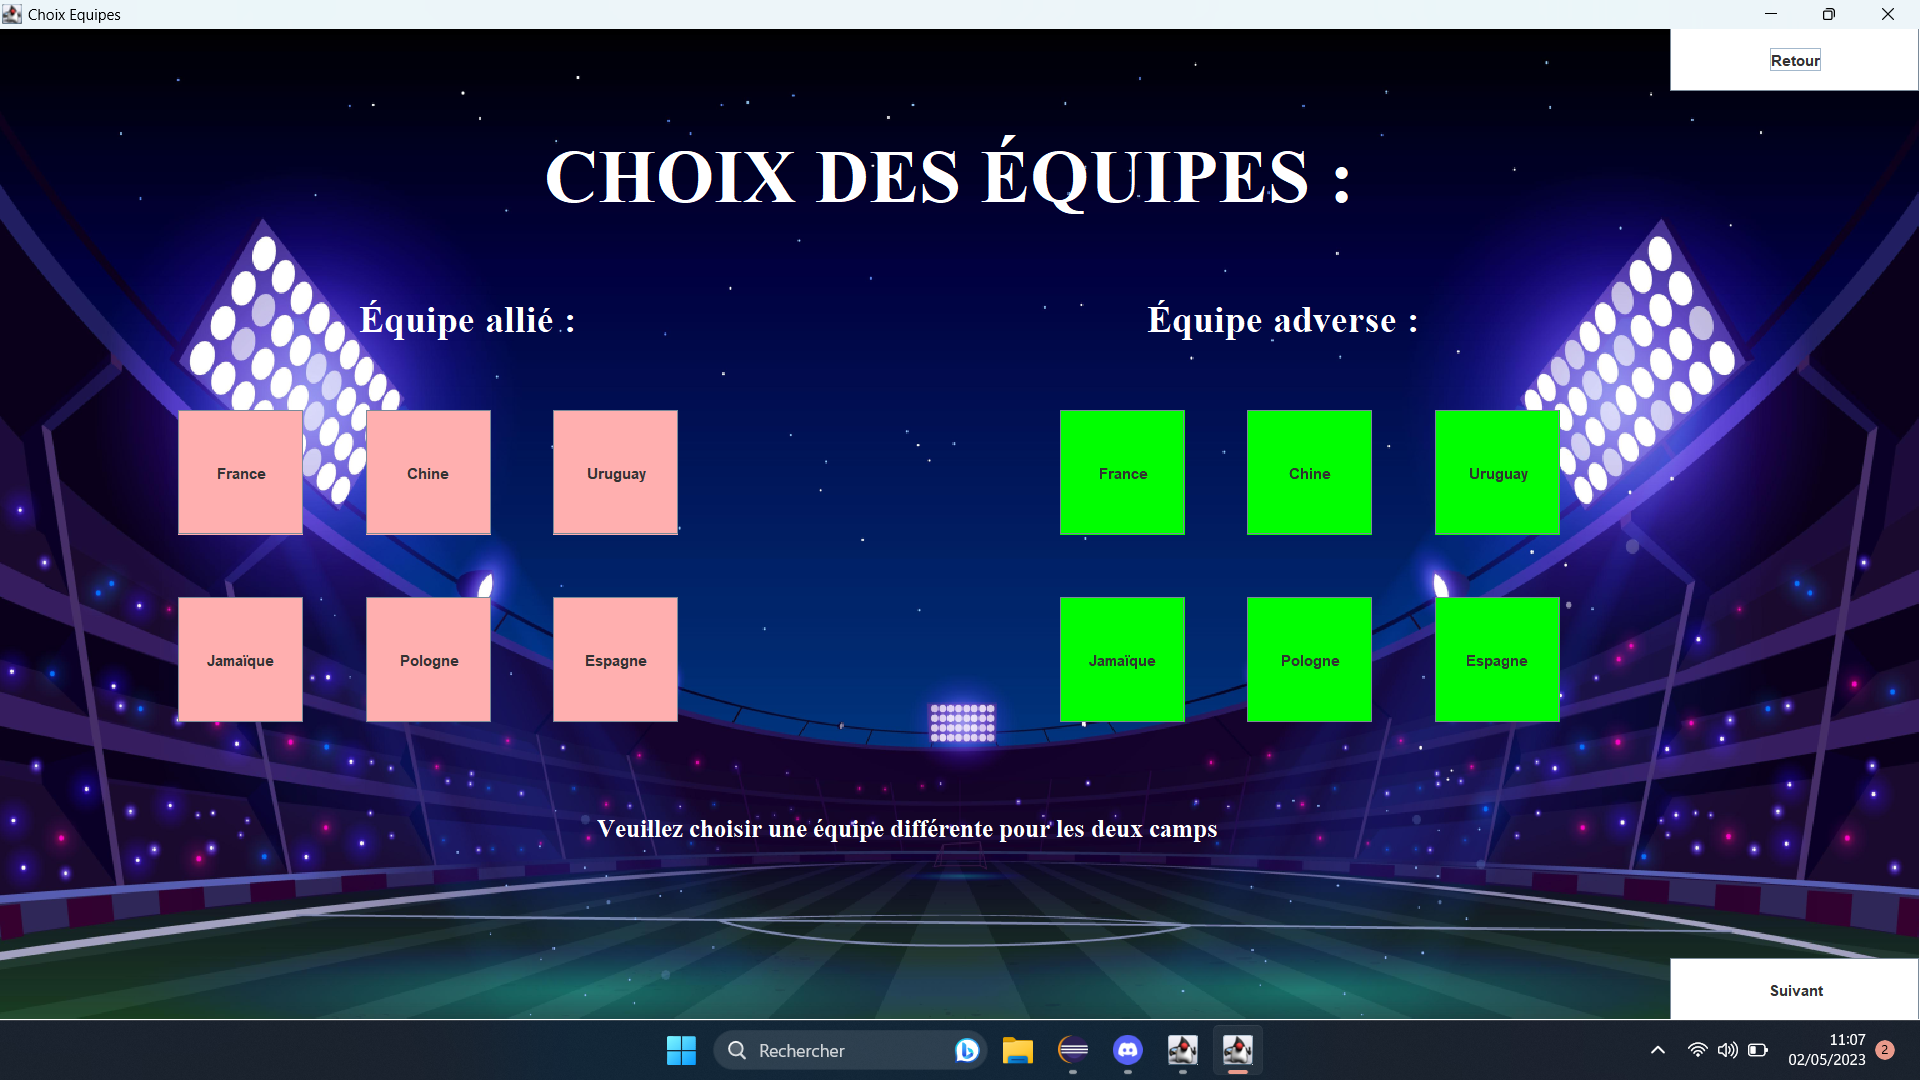
\includegraphics[width=12.82cm, height=8.2cm]{images/ChoixEquipe.png}
\caption{Choix Equipe}
\label{fig:choixEquipe}
\end{figure}

\paragraph{Page du choix des équipes}

\begin{itemize}
    \item \textbf{Retour :} 
        Si vous appuyez sur le bouton "Retour" situé en haut à droite, cela vous amènera à la page précédente qui est la page d'accueil.

    \vspace{15pt}

    \item \textbf{Les équipes :} 
        Au milieu de votre écran, vous voyez des noms de pays dans les cases roses et vertes, c'est ici que vous devez choisir le pays qui représentera votre équipe et celle de l'équipe adverse.

    \vspace{15pt}

    \item \textbf{Suivant :} 
        Si vous appuyez sur le bouton "Suivant" situé en bas à droite, cela vous amènera à la page suivante qui est la page de choix des postes, mais pour cela, vous devez choisir une équipe chacun.
        
    \vspace{15pt}
\end{itemize}

\begin{figure}[h]
\centering
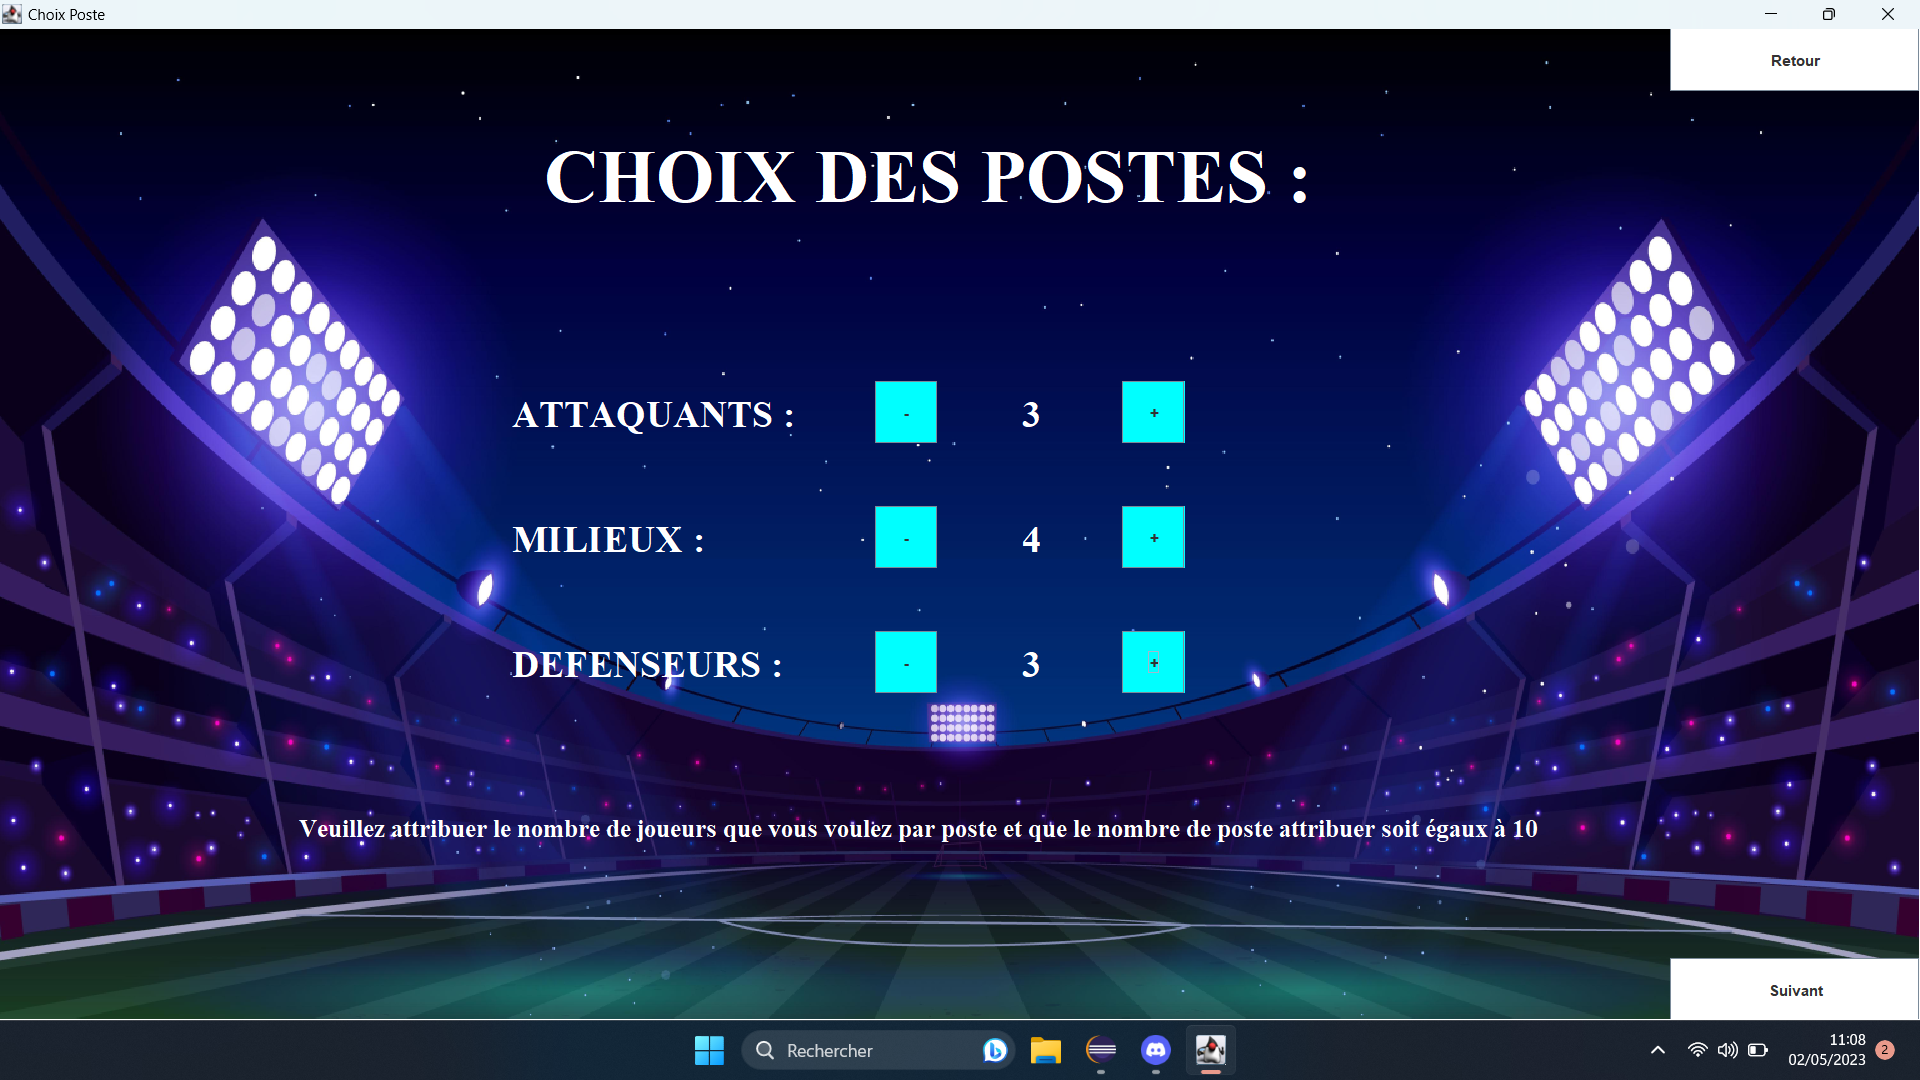
\includegraphics[width=12.82cm, height=8.2cm]{images/ChoixPoste.png}
\caption{Choix Poste}
\label{fig:choixPoste}
\end{figure}

    \vspace{15pt}

\paragraph{Page de la sélection de votre composition}

\begin{itemize}
    \item \textbf{Retour :} 
        Si vous appuyez sur le bouton "Retour" situé en haut à droite, cela vous amènera à la page précédente qui est la page de choix des équipes.

    \vspace{15pt}

    \item \textbf{Les postes :} 
        Au milieu de votre écran, vous voyez le nom des postes avec un bouton moins et plus, et au milieu un chiffre qui indique le nombre de personnes sur ce poste. Les boutons permettent d'ajouter ou d'enlever une personne à ce poste. Choisissez judicieusement votre composition, celle qui vous permettra d'obtenir la victoire.

    \vspace{15pt}

    \item \textbf{Suivant :} 
        Si vous appuyez sur le bouton "Suivant" situé en bas à droite, cela vous amènera à la page suivante qui est la page de choix des joueurs, mais pour cela, vous devez choisir 10 postes au total.
        
    \vspace{15pt}
\end{itemize}

\begin{figure}[h]
\centering
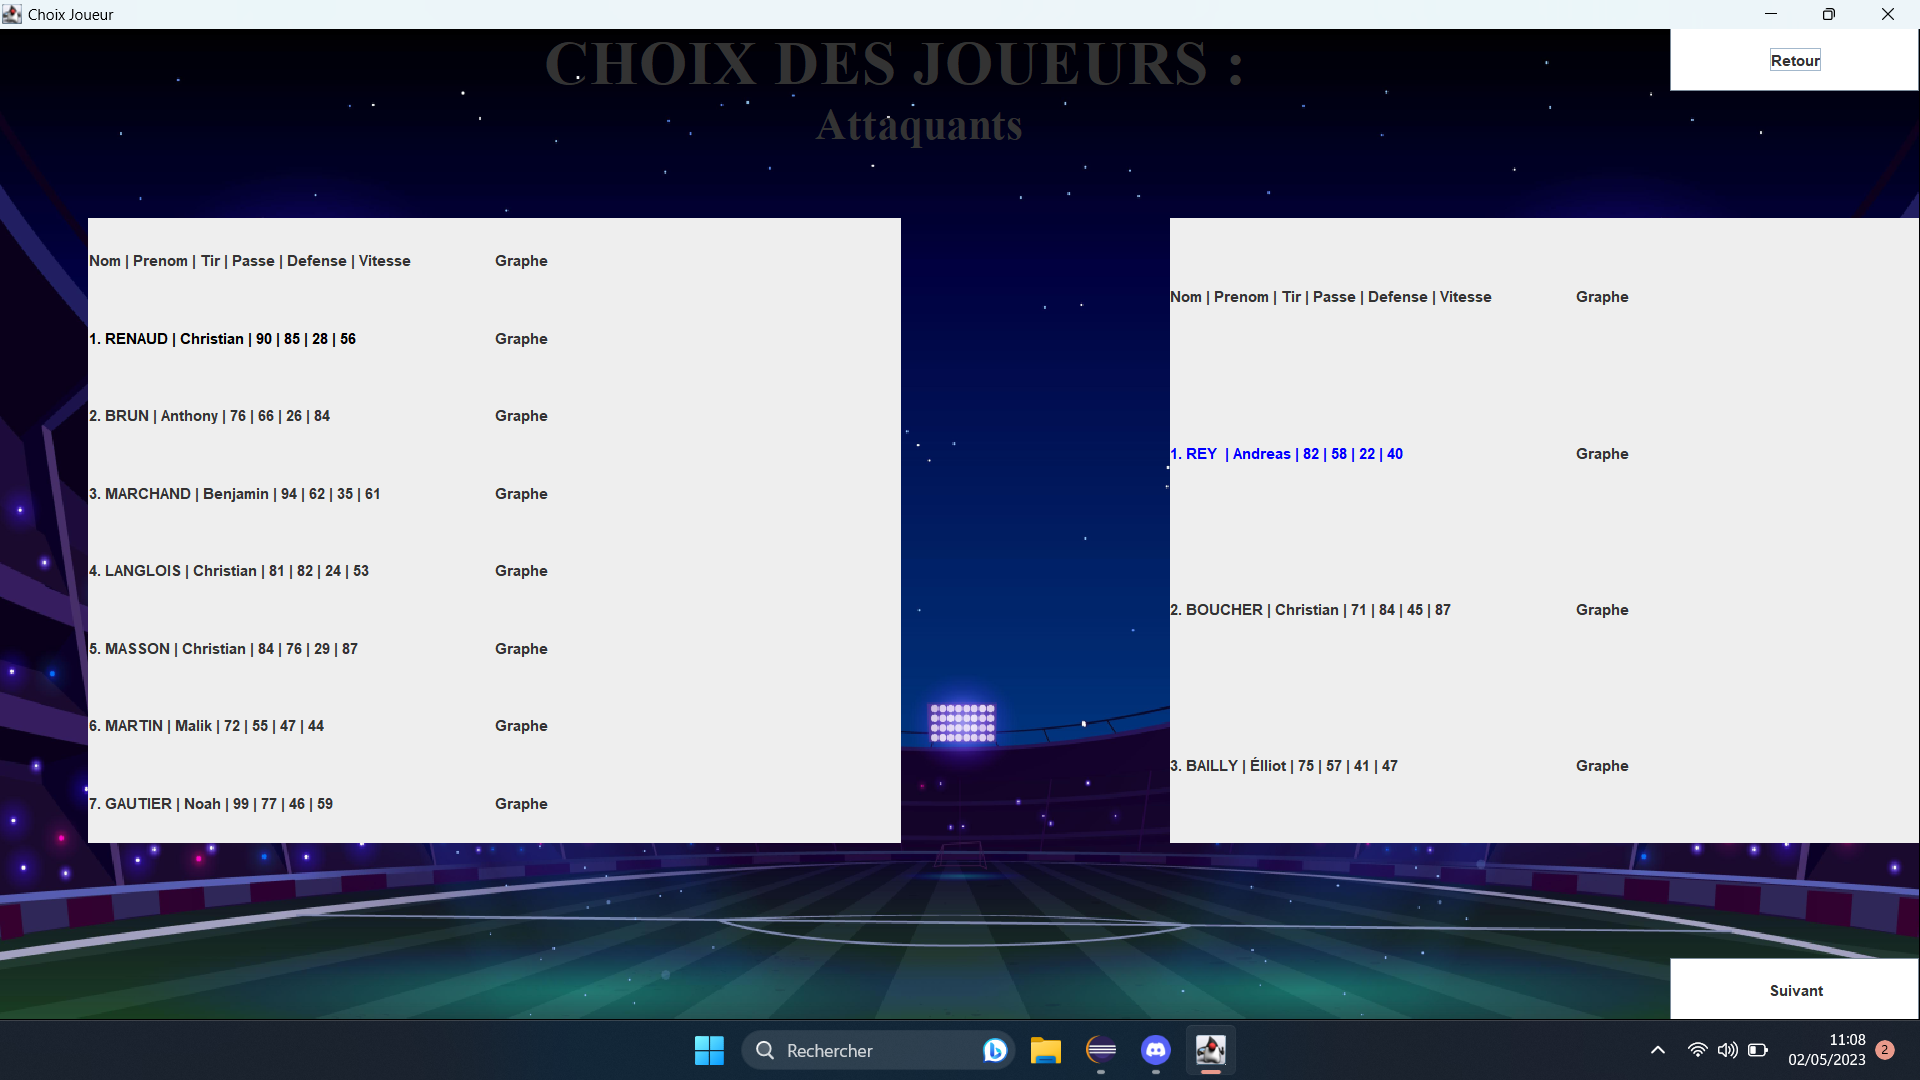
\includegraphics[width=12.82cm, height=8.2cm]{images/ChoixJoueur.png}
\caption{Choix Joueur}
\label{fig:choixJoueur}
\end{figure}

    \vspace{15pt}

\paragraph{Page de la sélection de vos joueurs}

\begin{itemize}
    \item \textbf{Retour :} 
        Si vous appuyez sur le bouton "Retour" situé en haut à droite, cela vous amènera à la page précédente qui est la page de choix des postes.

    \vspace{15pt}

    \item \textbf{Les joueurs :} 
         Au milieu de votre écran, vous voyez les joueurs avec leur nom, prénom et leurs statistiques liées à chacun. Vous devez choisir autant d'attaquants que de postes d'attaquant que vous avez choisis précédemment. Choisissez les meilleurs attaquants possible avec les meilleures statistiques possibles. Bien sûr, si vous vous êtes trompé d'attaquant, vous pouvez appuyer à nouveau dessus pour le faire partir.

    \vspace{15pt}

    \item \textbf{Suivant :} 
        Si vous appuyez sur le bouton "Suivant" situé en bas à droite, cela vous amènera à la page suivante qui est le match, mais pour cela, vous devez choisir le nombre d'attaquants que vous avez choisis. Ensuite, vous devez recommencer avec les milieux de terrain, puis les défenseurs et enfin le gardien.
        
    \vspace{15pt}
\end{itemize}















\subsection{Pendant le match}

\paragraph{}
    Dans cette sous-section, nous allons détailler les différentes actions qui seront réalisées durant le match, allant de la simulation d'un match de football aux statistiques calculées en temps réel, bien que l'utilisateur ne pourra rien faire étant donné que notre jeu n'est qu'une simulation.

\begin{figure}[h]
\centering
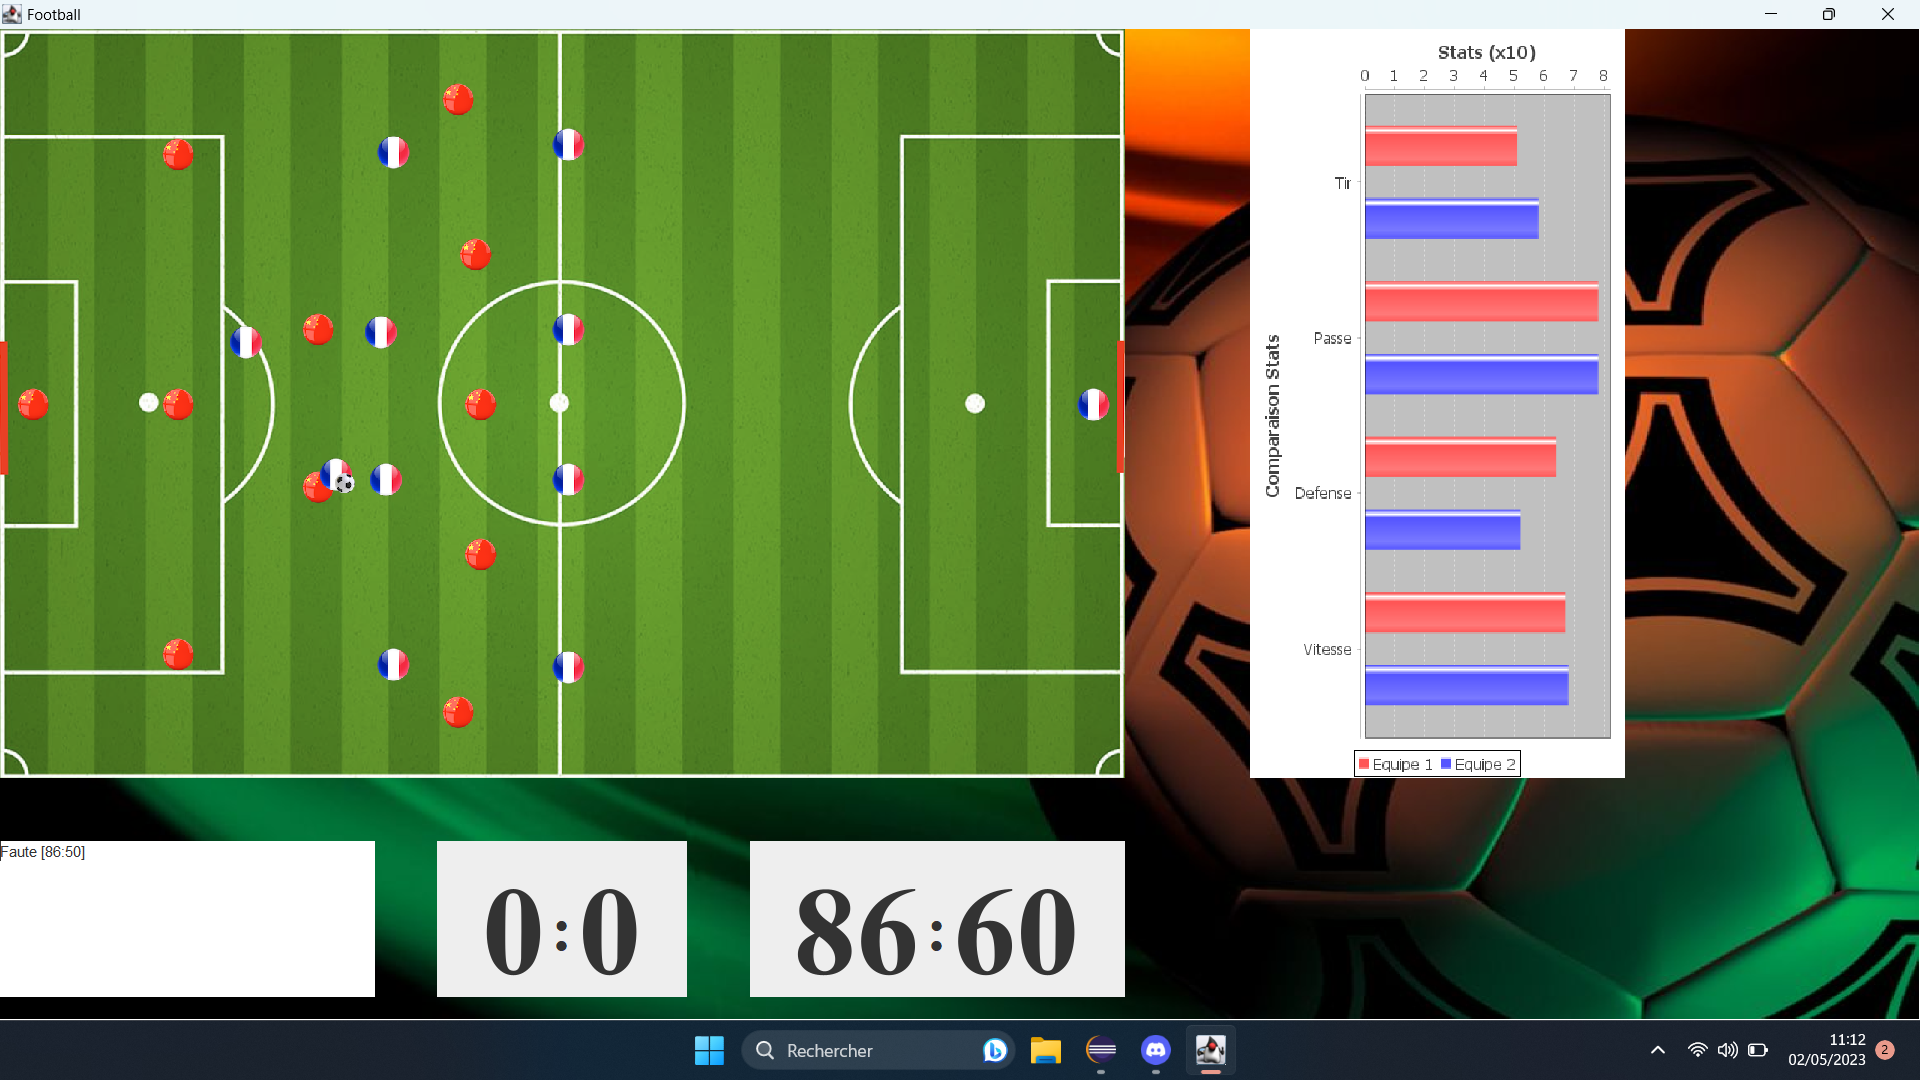
\includegraphics[width=12.82cm, height=8.2cm]{images/Match.png}
\caption{Match}
\label{fig:match}
\end{figure}

    \vspace{15pt}

\paragraph{Page de la simulation du match}

\begin{itemize}
    \item \textbf{En haut à gauche :} 
        Ceci est le match de football avec votre équipe positionnée à gauche et l'équipe adverse à droite. Maintenant, il ne vous reste plus qu'à regarder et encourager votre équipe. Bon match !

    \vspace{15pt}

    \item \textbf{À droite :} 
         Vous trouverez les moyennes des statistiques des joueurs en bleu pour votre équipe et en rouge pour l'équipe adverse à droite de votre écran.

    \vspace{15pt}

    \item \textbf{En bas} 
        \begin{itemize}
            
            \item \textbf{Les messages du jeux :}
                Le rectangle situé le plus à gauche est l'endroit où les actions spéciales telles que le corner, le but, etc., sont indiquées pour que vous puissiez suivre le match et comprendre ce qui se passe sans problème.
            
            \vspace{15pt}
            
            \item \textbf{Le score :}
                Le rectangle situé au milieu est l'endroit où les scores sont affichés. Ainsi, si votre équipe marque, vous pourrez le voir directement à cet endroit.

            \vspace{15pt}
            
            \item \textbf{Le temps :}
                Le rectangle à droite affiche le chronomètre pour vous permettre de savoir combien de temps il reste avant la fin du match. Lorsque le match est terminé, veuillez patienter 5 secondes et vous serez automatiquement redirigé vers la page des statistiques.
            
            \vspace{15pt}
        \end{itemize}

        
    \vspace{15pt}
\end{itemize}




    

\subsection{Après le match}

\paragraph{} 
    Dans cette sous-section, nous allons décrire l'affichage qui apparaîtra à la fin de la simulation de notre match de foot. Autrement dit, nous allons afficher les statistiques du match, le nom de l'équipe gagnante ainsi qu'un écran d'interaction avec l'utilisateur.

\begin{figure}[h]
\centering
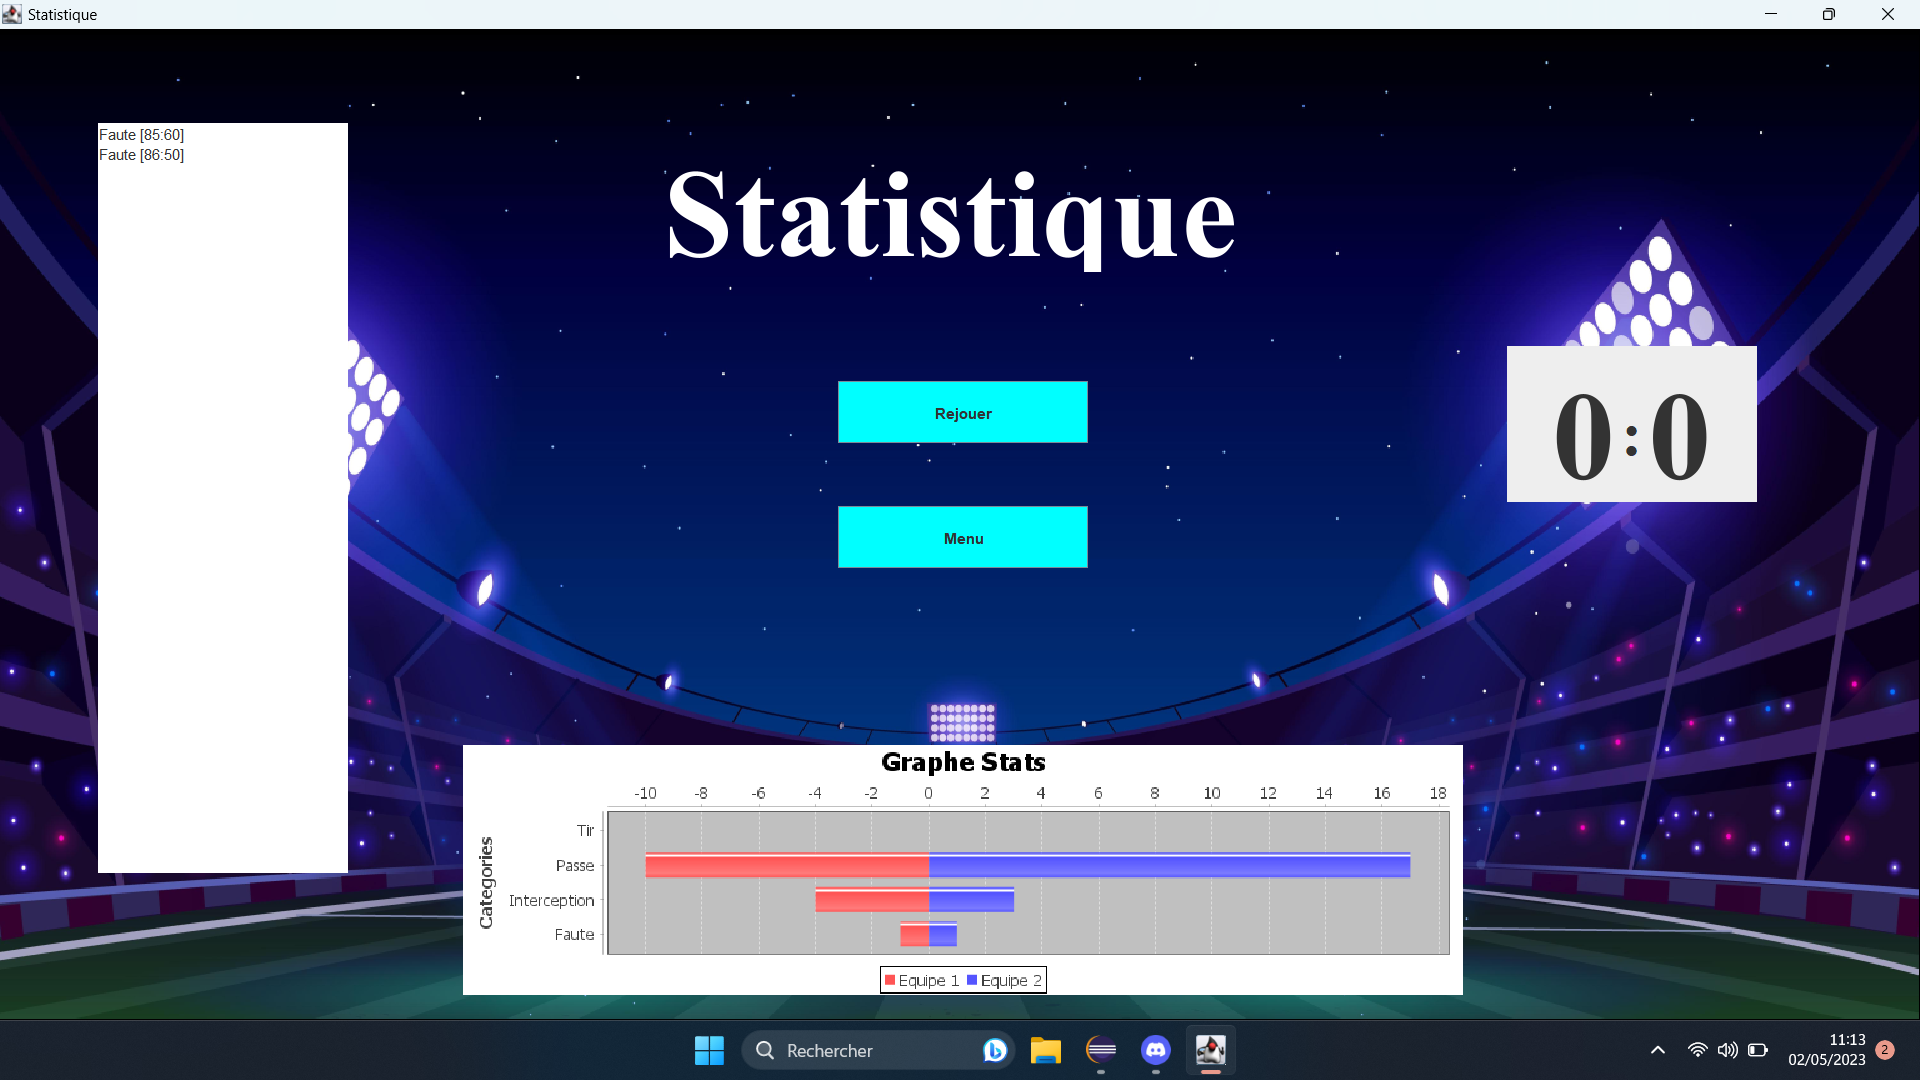
\includegraphics[width=12.82cm, height=8.2cm]{images/Statistiques.png}
\caption{Statistiques}
\label{fig:stats}
\end{figure}

    \vspace{15pt}

\paragraph{Page des statistiques}

\begin{itemize}
    \item \textbf{Rejouer :} 
        Si vous appuyez sur le bouton "Rejouer" il vous amènera directement sur la page du choix des équipes.

    \vspace{15pt}

    \item \textbf{Menu} 
         Si vous appuyez sur le bouton "Menu", cela vous amènera directement sur la page d'accueil.

    \vspace{15pt}

    \item \textbf{Les rectangles} 
        \begin{itemize}
            
            \item \textbf{Les messages du jeux :}
                Le rectangle situé à gauche est l'endroit où toutes les actions spéciales du match telles que le corner, le but, etc., sont indiquées afin que vous puissiez suivre le match et comprendre ce qui se passe sans problème.
            
            \vspace{15pt}
            
            \item \textbf{Le score :}
                Le rectangle situé à droite est l'endroit où les scores de fin de match sont affichés.

            \vspace{15pt}
            
            \item \textbf{Les statistiques}
                Le rectangle en bas affiche les statistiques de fin de match telles que le nombre de tirs, le nombre de passes, etc.
            
            \vspace{15pt}
        \end{itemize}
        
    \vspace{15pt}
\end{itemize}
\newpage
\section{Déroulement du projet}
\label{sec:deroulement}

Dans cette section, nous décrivons comment le projet a été réalisé en équipe : la répartition des tâches, la synchronisation du travail en membres de l'équipe, etc.

\subsection{Répartition des taches et organisation globale}

\paragraph{}
    Dans un premier temps, nous détaillerons la répartition des différentes taches au sein du groupe et leur espacement dans le temps tel quelle fut imaginer.

\begin{center}
\begin{tabular}{ |c|c|c|c|c|c| } 
 \hline
   & Boyan & Romain & Guillaume & temps estimé & temps réel\\ 
 \hline\hline
   Cahier des charges & V & V & V & 4 jours &1 semaine\\ 
 \hline
  Conception graphique & V & V & V & 2 jours & 2 jours\\ 
 \hline
 Déplacement de la balle & X & X & V & 1 semaine & 2 semaine\\ 
 \hline
 Gestion des actions & V & V & X & 2 semaines &2 semaines\\
 \hline
 Réalisation des actions & V & V & X & 2 semaines & 3 semaines\\
 \hline
 Classe de donnée & V & V & V & 5 jours & 4 jours\\
 \hline
 IHM & V & X & X & Tout le long & Tous le long\\
 \hline
  Chart & X & V & V & 2 jours & 2 jours\\
 \hline
   CNP & V & V & V & 4 jours & 5 jours\\
 \hline
    Présentation technique & V & V & V & 5 jours & 5 jours\\
 \hline
 Rapport & V & V & V & 3 jours & 3 jours\\  
 \hline
\end{tabular}
\end{center}

\paragraph{}
    Dans un second temps, nous comparerons l'estimation à la réalité du projet.
    
\paragraph{}
    La différence de temps peut être une source de frustration dans tout projet. Cependant, la solution pour y remédier est simple : il suffit de faire preuve de réalisme et de prudence dès le début. En effet, nous avons reconnu que notre ambition excessive et notre manque de prévoyance nous ont empêchés de faire face efficacement aux difficultés imprévues, qui ont considérablement ralenti notre progression. Pour éviter cela, il est crucial de prendre en compte les risques potentiels dès le début du projet et de planifier des marges de manœuvre en termes de temps pour les imprévus. En outre, nous devons adopter une approche plus prudente quant à nos attentes et objectifs, en veillant à ce qu'ils soient réalistes et réalisables dans les délais impartis. En adoptant cette approche, nous pourrons minimiser les risques et les retards, tout en garantissant la qualité et la réussite de notre projet.
    
\subsection{Défis rencontrés}

\paragraph{}
    Ici, nous décrirons les différentes problématiques rencontrée tel que le fait de programmer à 3 sur un projet, etc.

\paragraph{}
    Parmi les nombreux défi rencontrés tout au long de la réalisation du projet, on retrouve principalement la collaboration à trois sur un projet aussi minutieux. En effet, il n’a pas toujours été évident de se repartir les tâches ou encore de programmer chacun de son coté sur le même projet simultanément.
\paragraph{}
    De plus, la gestion du temps fait également l’objet d’un défi conséquent dans l’aboutissement du projet. Il est clair que nous avons souvent eu à se re concentrer sur le projet de façon assidu afin de ne pas prendre trop de retard, car le semestre est passé très vite et il est bien plus simple de prendre du retard que d'en rattraper.
\paragraph{}
    Également, de gros défis algorithmique ont été rencontrés et surmontés. Une simulation de jeu de foot est évidemment pas mince affaire. Ainsi, nous avons tous eu a se creuser la tête un grands nombres de fois afin de surmonter ces défis et réaliser un jeu de foot réaliste et parfaitement fonctionnel.
\paragraph{}
    En fin de compte, notre plus grand défi a été de créer un projet qui reflète notre vision et notre identité, tout en répondant aux attentes et aux besoins de notre projet. Nous avons travaillé dur pour concevoir un produit qui nous plaît et dont nous sommes fiers, tout en étant convaincus qu'il soit un minimum convaincant. Cela n'a pas été facile, car il y avait des compromis à faire et des choix à faire tout au long du processus de développement. Cependant, nous avons pris soin d'écouter les commentaires et les retours de nos proches pour prendre des décisions éclairées et garantir la qualité de notre projet. Nous sommes convaincus que nous avons réussi à créer un produit qui répond à nos exigences et qui rempli une bonne parti des consignes.
\newpage
\section{Conclusion et perspectives}
\label{sec:conclusion}

\noindent Dans cette section, nous résumerons la réalisation du projet et nous présenterons également les extensions et améliorations possibles du projet de façons objectives et qualitatives. 

\subsection{Achèvement du projet}

\paragraph{}
    Dans cette sous-section, nous détaillerons le niveau d'achèvement de notre projet, par rapport aux attentes de bases, et aux objectifs qui nous avions été fixées au préalable dans le cahier des charges (\ref{sec:specification}).

    Le fait que le projet soit à 80\% terminé est une bonne nouvelle, car cela signifie que la majeure partie du travail a déjà été effectuée. Bien qu'il reste quelques petits détails à régler, comme l'ajout de l'endurance des joueurs et des pouvoirs inclus dans le cahier des charges, il est important de reconnaître que ce retard a permis d'améliorer certaines parties du projet. En effet, en prenant le temps de peaufiner les détails déjà en place, l'équipe a pu affiner les fonctionnalités existantes pour les rendre plus performantes et plus efficaces. De plus, cela a également permis de mieux comprendre les besoins des utilisateurs et de s'adapter en conséquence. Ainsi, même si le projet n'est pas encore complètement terminé, cette situation a en fait permis d'optimiser son potentiel et de répondre aux attentes des utilisateurs de manière plus satisfaisante.
    

\subsection{Points d'améliorations possibles}

\paragraph{}
    Dans cette sous-section, nous exprimerons les possibles points d'améliorations de notre projet, au vu de notre réalisation et en lien avec notre niveau d'achèvement.

\paragraph{}
    Tout d'abord, on pense que l'un des points faibles de notre projet est le manque de super pouvoirs. Contrairement à ce qu'on avait initialement prévu, on a décidé de ne pas inclure de super pouvoirs dans le jeu, ce qui pourrait limiter la variété de jeu et de stratégies que les joueurs peuvent utiliser. En conséquence, on va travailler sur des alternatives pour permettre aux joueurs d'explorer différents styles de jeu et de stratégies sans l'utilisation de super pouvoirs.

De plus, on est conscient que le manque de choix stratégique dans le jeu peut également être un point faible. Bien qu'on ait ajouté quelques options de stratégie telles que les changements de formation et les ajustements tactiques, on reconnaît que cela pourrait ne pas être suffisant pour les joueurs qui cherchent à personnaliser leur jeu. Pour améliorer cela, on va travailler sur l'ajout de plus d'options de stratégie, telles que les substitutions et les remplacements pour permettre aux joueurs de s'adapter rapidement à la situation sur le terrain. Cependant, un autre aspect lié à l'absence de choix stratégique que nous avons identifié est le manque de cartons jaunes et rouges dans le jeu. Nous allons travailler sur l'ajout de ces éléments pour une expérience de jeu plus réaliste et immersive.

Au surplus, un autre point faible que nous avons identifié est le manque de cartons jaunes et rouges dans le jeu. Les sanctions pour les fautes sont une partie importante du football, et sans elles, le jeu peut sembler moins réaliste et moins engagé. Nous allons travailler sur l'ajout de cartons jaunes et rouges pour les fautes commises par les joueurs, afin de mieux refléter les règles et les normes du football.

En outre, nous avons également réalisé que les remplaçants ne servent pas à grand-chose dans notre projet. Bien qu'ils soient inclus dans le jeu, leur utilité est limitée car ils ne peuvent pas être utilisés pour influencer directement le jeu. Pour résoudre ce problème, nous allons travailler sur l'ajout de plus d'options de remplacement et de substitutions pour permettre aux joueurs de mieux gérer leur équipe et de s'adapter à la situation sur le terrain. Nous pensons que cela permettra aux joueurs de mieux utiliser les remplaçants pour influencer le jeu et ainsi améliorer l'expérience globale de jeu.

Un autre point faible de notre projet est le manque de style et de réalisme dans le jeu. Bien qu'on ait ajouté quelques éléments visuels et sonores pour renforcer l'ambiance du jeu, on reconnaît que cela pourrait ne pas être suffisant pour créer une expérience de jeu véritablement immersive. Pour améliorer cela, on va travailler sur l'ajout de plus d'options de personnalisation pour les joueurs, les équipes et les stades. On va également travailler sur la physique du ballon et des joueurs pour rendre le jeu plus réaliste. Nous avons également remarqué que les remplaçants ne servent actuellement à rien dans le jeu, nous allons donc travailler sur l'ajout de fonctionnalités pour permettre aux joueurs de mieux gérer leur banc de remplaçants.

Enfin, on reconnaît que le manque de fluidité dans le jeu peut être un point faible. On est conscient que les ralentissements et les latences peuvent affecter l'expérience de jeu des joueurs. Pour résoudre ce problème, on va travailler sur l'optimisation du jeu en utilisant des serveurs dédiés et en offrant des options de personnalisation pour permettre aux joueurs d'optimiser les performances selon leur matériel.

En conclusion, bien qu'on ait créé un projet de simulation de football intéressant, il y a plusieurs points que l'on reconnaît comme étant des points faibles. Cependant, on est déterminé à améliorer ces points faibles en ajoutant plus de super pouvoirs, d'options de stratégie, de personnalisation et d'optimisation pour garantir une expérience de jeu plus immersive et agréable pour les joueurs. Nous sommes conscients que cela nécessite un travail conséquent, mais nous sommes persuadés que cela améliorera considérablement la qualité de notre jeu.




\end{document}
